\documentclass{assignment}
\usepackage[pdftex]{graphicx} 
\usepackage{xcolor}
\definecolor{LightGray}{gray}{0.95}
%\usepackage{fancyvrb, minted} 
\usepackage[a4paper, margin = 2.5cm]{geometry} 
\usepackage[T1]{fontenc} 
% set figure path 
\graphicspath{figures}

\usepackage{amsmath, amsfonts, amssymb} 
\usepackage{hyperref, url}  
\usepackage{fancyhdr}
\usepackage{setspace}
\onehalfspacing

\usepackage{float}
\usepackage{subcaption}
\usepackage{listingsutf8}

\usepackage{xcolor}

\definecolor{codegreen}{rgb}{0,0.6,0}
\definecolor{codegray}{rgb}{0.5,0.5,0.5}
\definecolor{codepurple}{rgb}{0.58,0,0.82}
\definecolor{backcolour}{rgb}{0.95,0.95,0.92}

\lstdefinestyle{mystyle}{
    backgroundcolor=\color{backcolour},   
    commentstyle=\color{codegreen},
    keywordstyle=\color{magenta},
    numberstyle=\tiny\color{codegray},
    stringstyle=\color{codepurple},
    basicstyle=\ttfamily\footnotesize,
    breakatwhitespace=false,         
    breaklines=true,                 
    captionpos=b,                    
    keepspaces=true,                 
    numbers=left,                    
    numbersep=5pt,                  
    showspaces=false,                
    showstringspaces=false,
    showtabs=false,                  
    tabsize=2
}

\lstset{style=mystyle}

\student{Ahmet Akman 2442366}                             
\semester{Spring 2024}                            
\date{\today}                                   

\courselabel{EE449}          
\exercisesheet{Homework 2}{Report}  

\school{Middle East Technical University}        
\university{Electrical and Electronics Engineering}        

%%%%%%%%%%%%%%%%%%%%%%%%%%%%%%%%%%%%%%%%%%-DOCUMENT-%%%%%%%%%%%%%%%%%%%%%%%%%%%%%%%%%%%%%%%%%%%%

\begin{document}
\section{Experimental Work}
The parameter set provided in Table \ref{tab:parameter_sweep} is used to perform qualitative analysis of different evoulationary algorithm parameters.

\begin{table}[htbp!]
    \centering
    \caption{Parameter set used in this experiment.}
    \label{tab:parameter_sweep}
    \begin{tabular}{|c|ccccc|}
    \hline
    \textbf{Parameter}                      & \multicolumn{5}{c|}{\textbf{Values}}                                                                                                       \\ \hline
    \textless{}num\_inds\textgreater{}      & \multicolumn{1}{c|}{5}        & \multicolumn{1}{c|}{10}              & \multicolumn{1}{c|}{\textbf{20}}  & \multicolumn{1}{c|}{40}   & 60  \\ \hline
    \textless{}num\_genes\textgreater{}     & \multicolumn{1}{c|}{15}       & \multicolumn{1}{c|}{30}              & \multicolumn{1}{c|}{\textbf{50}}  & \multicolumn{1}{c|}{80}   & 120 \\ \hline
    \textless{}tm\_size\textgreater{}       & \multicolumn{1}{c|}{2}        & \multicolumn{1}{c|}{\textbf{5}}      & \multicolumn{1}{c|}{8}            & \multicolumn{1}{c|}{16}   &     \\ \hline
    \textless{}frac\_elites\textgreater{}   & \multicolumn{1}{c|}{0.04}     & \multicolumn{1}{c|}{\textbf{0.2}}    & \multicolumn{1}{c|}{0.35}         & \multicolumn{1}{c|}{}     &     \\ \hline
    \textless{}frac\_parents\textgreater{}  & \multicolumn{1}{c|}{0.15}     & \multicolumn{1}{c|}{0.3}             & \multicolumn{1}{c|}{\textbf{0.6}} & \multicolumn{1}{c|}{0.75} &     \\ \hline
    \textless{}mutation\_prob\textgreater{} & \multicolumn{1}{c|}{0.1}      & \multicolumn{1}{c|}{\textbf{0.2}}    & \multicolumn{1}{c|}{0.4}          & \multicolumn{1}{c|}{0.75} &     \\ \hline
    \textless{}mutation\_type\textgreater{} & \multicolumn{1}{c|}{unguided} & \multicolumn{1}{c|}{\textbf{guided}} & \multicolumn{1}{c|}{}             & \multicolumn{1}{c|}{}     &     \\ \hline
\end{tabular}
\end{table}

\subsection{Default Parameter Set}
Let us first start with the results of default parameter set provided in the homework description to be used as a baseline throughout the experiment. Figure \ref{fig:default} shows the plots associated with the fitness value of the best individual. The default parameter set is indicated as bold in Table \ref{tab:parameter_sweep}.


\begin{figure}[H]
    \begin{subfigure}{0.5\textwidth}
        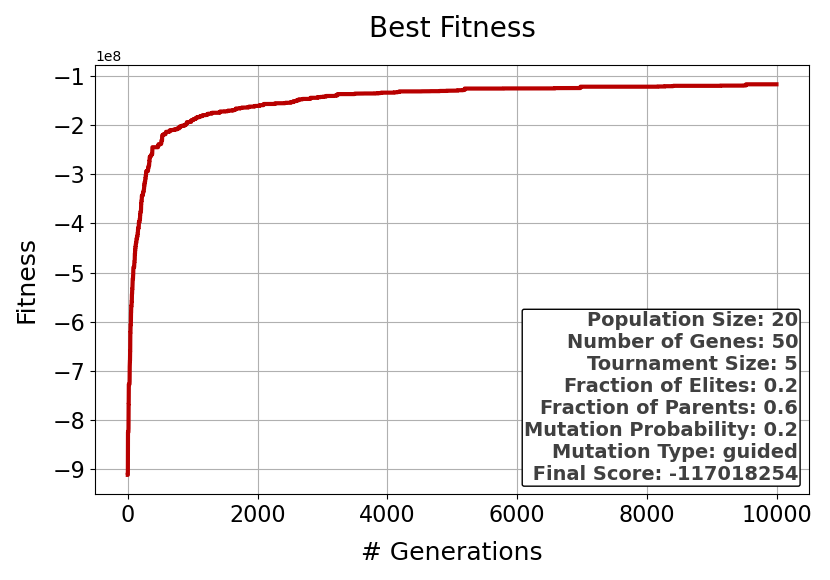
\includegraphics[width=\textwidth]{figures/best_fitness_output_20_50_5_0.2_0.6_0.2_guided.png}
        \caption{From first generation to 10000th generation.}
    \end{subfigure}\hfill
    \begin{subfigure}{0.5\textwidth}
        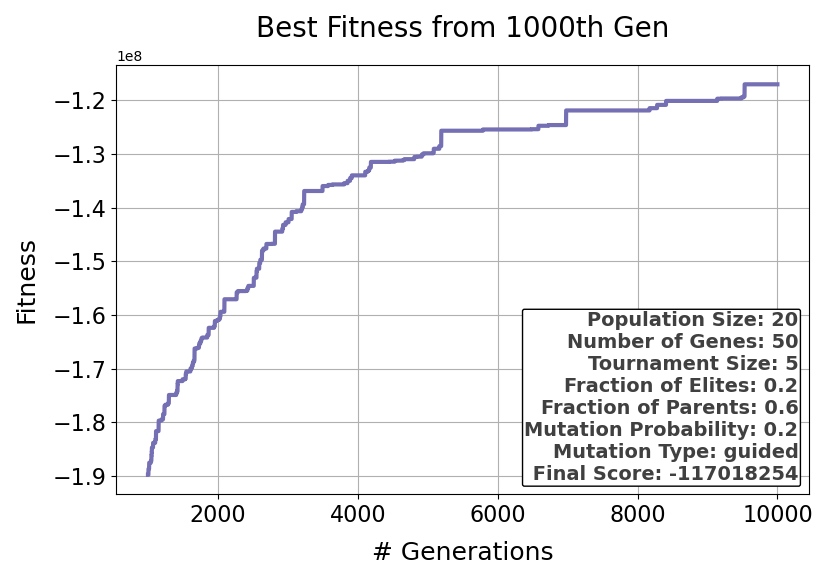
\includegraphics[width=\textwidth]{figures/best_fitness_1000_output_20_50_5_0.2_0.6_0.2_guided.png}
        \caption{From 1000th generation to 10000th generation.}
    \end{subfigure}
    \caption{Fitness curves.}
    \label{fig:default}
\end{figure}
The figures tells us that in the first 1000 generations, the fitness value of the best individual increases rapidly. However, after the 1000th generation, the increase in fitness value slows down. However, the fitness value of the best individual is still increasing and we can see this from the figure on the right. That means the algorithm continue to improve even after rapid jump.

The Figure \ref{fig:default_image} shows the evolution of the best individual quantitatively. The first image is the image in 1000th generation and the last image is the final image. The images in between are the images of the best individual in every 1000 generation. The images are generated by overlaying the circle represented by each gene one by one on the plain white image as instructed.


\begin{figure}[!htb]
    \centering
    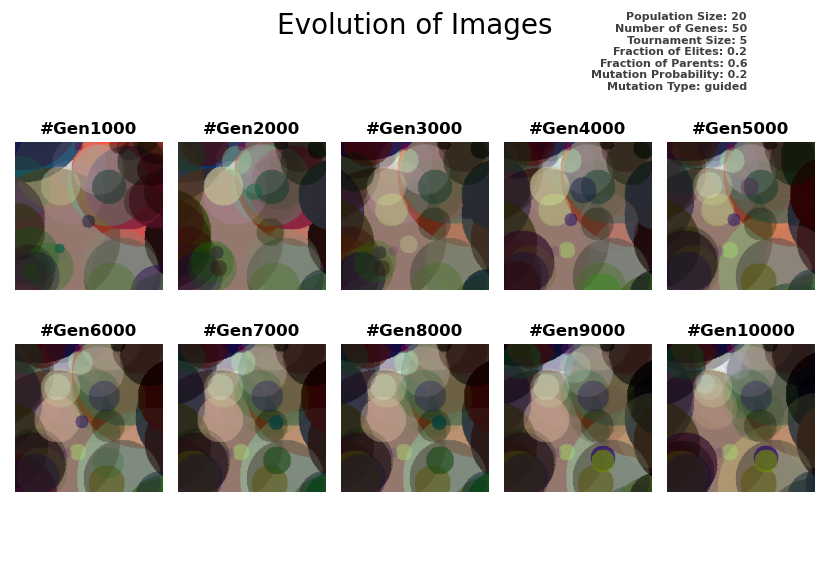
\includegraphics[width=0.9\textwidth]{figures/images_output_20_50_5_0.2_0.6_0.2_guided.png}
    \caption{Quantitative evolution of the best individual in the population.}
    \label{fig:default_image}
\end{figure}

\subsection{Number of Individuals}
Let us first provide necessary plots for the parameter \textless{}num\_inds\textgreater{}. 
\subsubsection{5 Individuals}
Figure \ref{fig:5inds} shows the plots associated with the fitness value of the best individual for 5 individuals.

\begin{figure}[H]
    \begin{subfigure}{0.5\textwidth}
        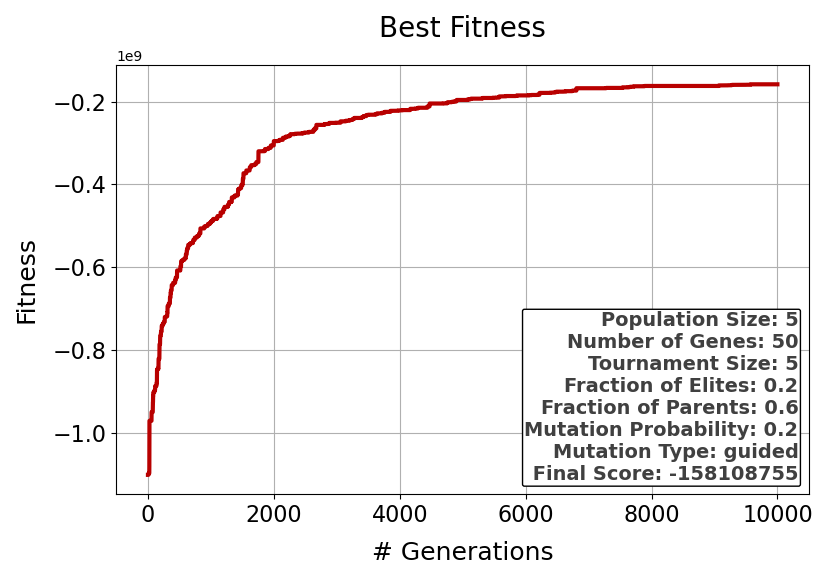
\includegraphics[width=\textwidth]{figures/best_fitness_output_5_50_5_0.2_0.6_0.2_guided.png}
        \caption{From first generation to 10000th generation.}
    \end{subfigure}\hfill
    \begin{subfigure}{0.5\textwidth}
        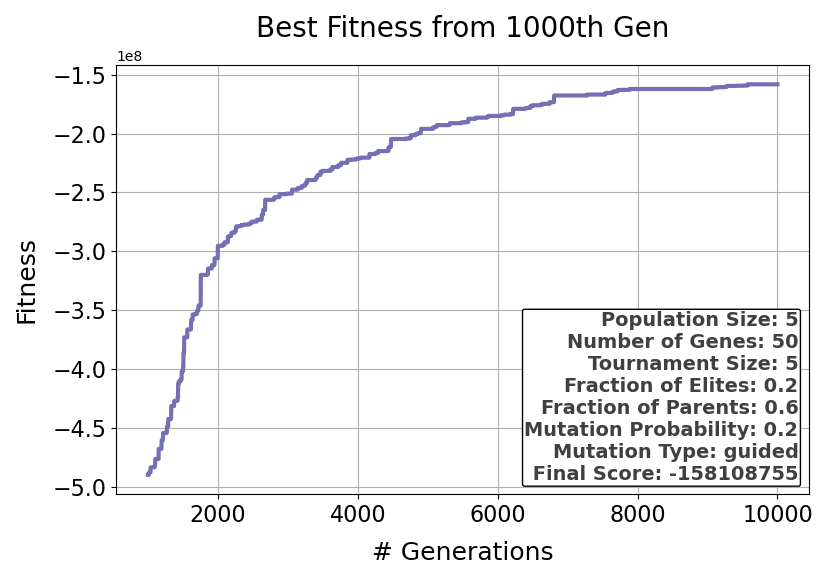
\includegraphics[width=\textwidth]{figures/best_fitness_1000_output_5_50_5_0.2_0.6_0.2_guided.png}
        \caption{From 1000th generation to 10000th generation.}
    \end{subfigure}
    \caption{Fitness curves for 5 individuals.}
\label{fig:5inds}
\end{figure}

The Figure \ref{fig:5inds_image} shows the evolution of the best individual quantitatively for 5 individuals.

\begin{figure}[!htb]
    \centering
    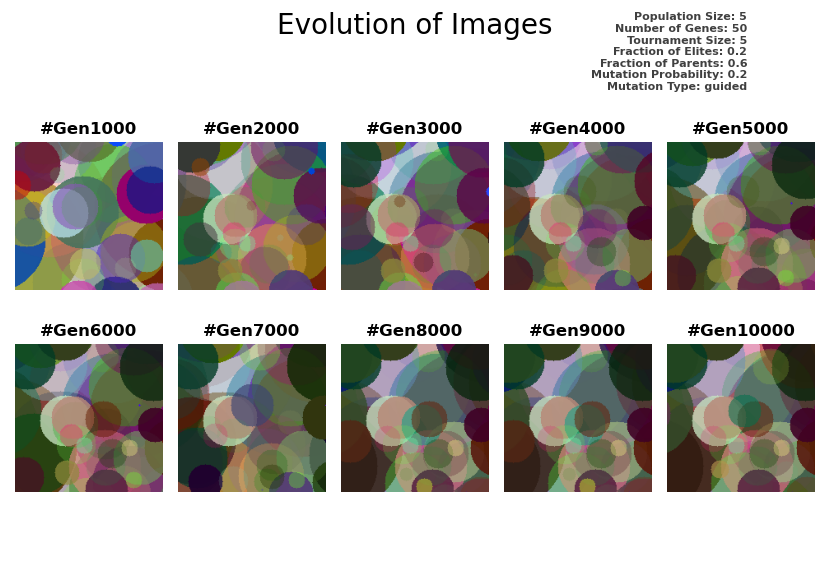
\includegraphics[width=0.9\textwidth]{figures/images_output_5_50_5_0.2_0.6_0.2_guided.png}
    \caption{Quantitative evolution of the best individual in the population for 5 individuals.}
    \label{fig:5inds_image}
\end{figure}

\subsubsection{10 Individuals}
Figure \ref{fig:10inds} illustrates the plots associated with the fitness value of the best individual for 10 individuals.

\begin{figure}[H]
    \begin{subfigure}{0.5\textwidth}
        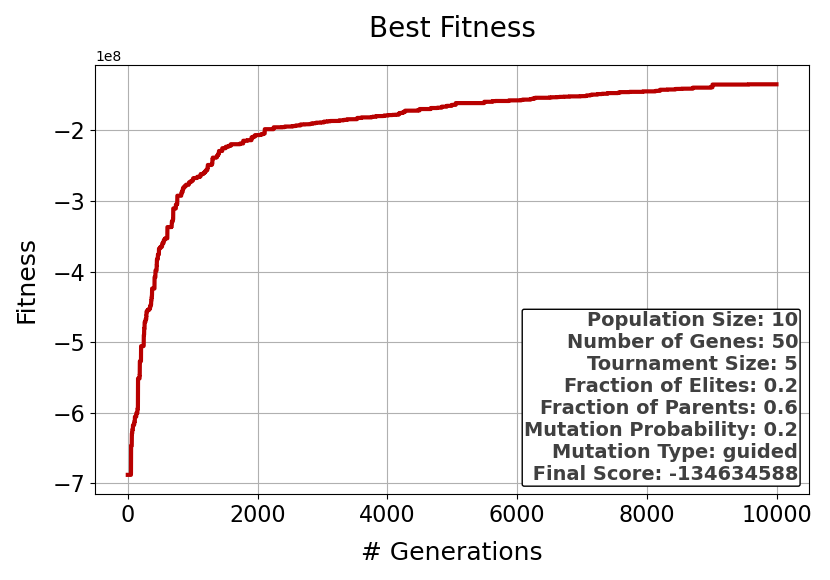
\includegraphics[width=\textwidth]{figures/best_fitness_output_10_50_5_0.2_0.6_0.2_guided.png}
        \caption{From first generation to 10000th generation.}
    \end{subfigure}\hfill
    \begin{subfigure}{0.5\textwidth}
        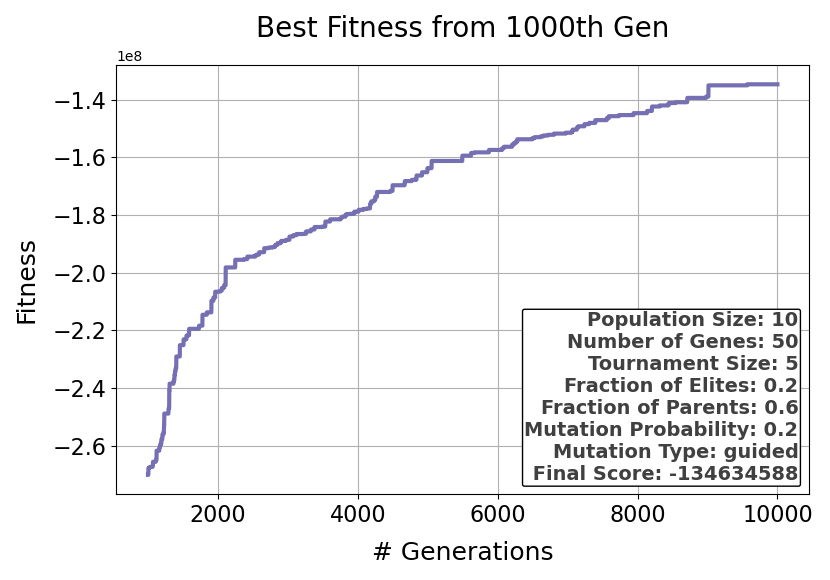
\includegraphics[width=\textwidth]{figures/best_fitness_1000_output_10_50_5_0.2_0.6_0.2_guided.png}
        \caption{From 1000th generation to 10000th generation.}
    \end{subfigure}
    \caption{Fitness curves for 10 individuals.}
\label{fig:10inds}
\end{figure}

The Figure \ref{fig:10inds_image} shows the evolution of the best individual quantitatively for 10 individuals.

\begin{figure}[!htb]
    \centering
    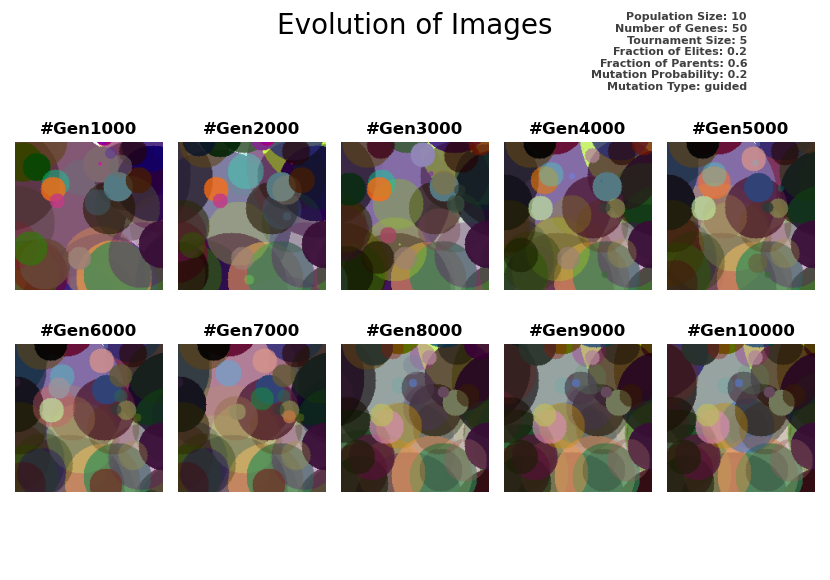
\includegraphics[width=0.9\textwidth]{figures/images_output_10_50_5_0.2_0.6_0.2_guided.png}
    \caption{Quantitative evolution of the best individual in the population for 10 individuals.}
    \label{fig:10inds_image}
\end{figure}

\subsubsection{40 Individuals}

Figure \ref{fig:40inds} shows the plots associated with the fitness value of the best individual for 40 individuals.

\begin{figure}[H]
    \begin{subfigure}{0.5\textwidth}
        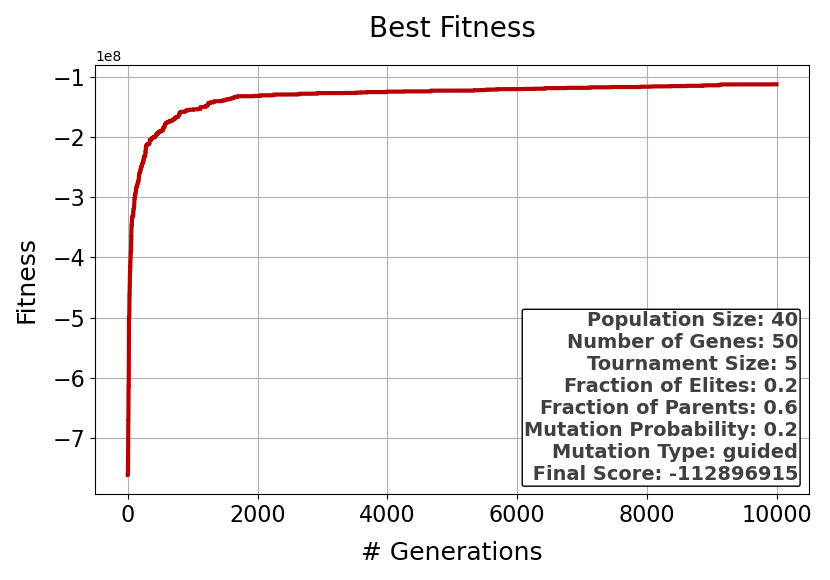
\includegraphics[width=\textwidth]{figures/best_fitness_output_40_50_5_0.2_0.6_0.2_guided.png}
        \caption{From first generation to 10000th generation.}
    \end{subfigure}\hfill
    \begin{subfigure}{0.5\textwidth}
        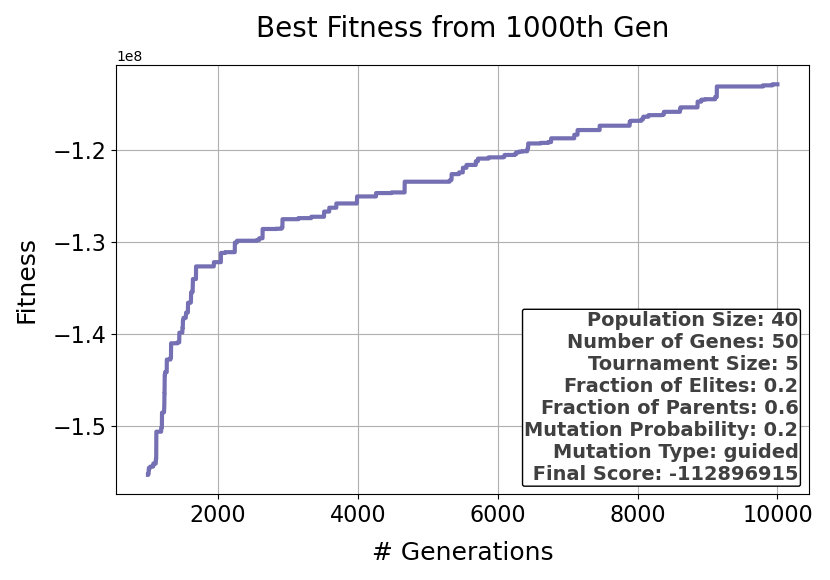
\includegraphics[width=\textwidth]{figures/best_fitness_1000_output_40_50_5_0.2_0.6_0.2_guided.png}
        \caption{From 1000th generation to 10000th generation.}
    \end{subfigure}
    \caption{Fitness curves for 40 individuals.}
\label{fig:40inds}
\end{figure}

The Figure \ref{fig:40inds_image} indicates the evolution of the best individual quantitatively for 40 individuals.

\begin{figure}[!htb]
    \centering
    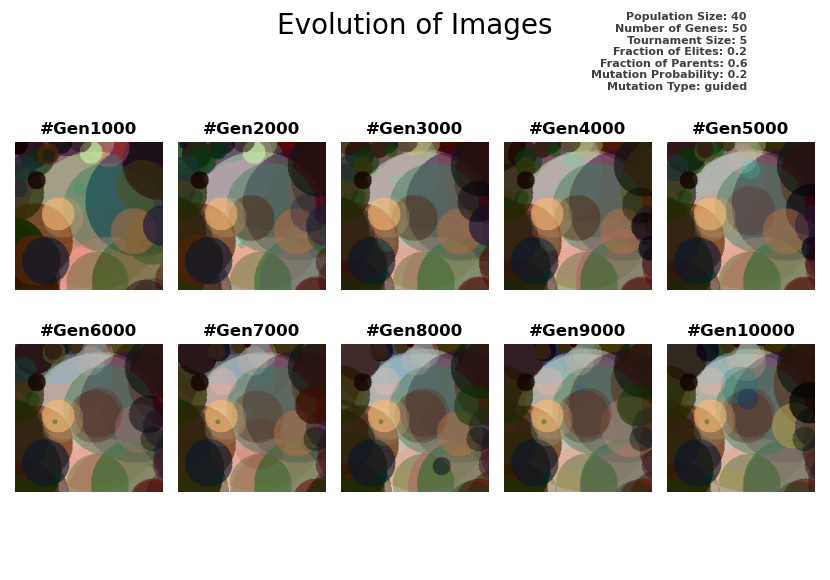
\includegraphics[width=0.9\textwidth]{figures/images_output_40_50_5_0.2_0.6_0.2_guided.png}
    \caption{Quantitative evolution of the best individual in the population for 40 individuals.}
    \label{fig:40inds_image}
\end{figure}

\subsubsection{60 Individuals}

Figure \ref{fig:60inds} shows the plots associated with the fitness value of the best individual for 60 individuals.

\begin{figure}[H]
    \begin{subfigure}{0.5\textwidth}
        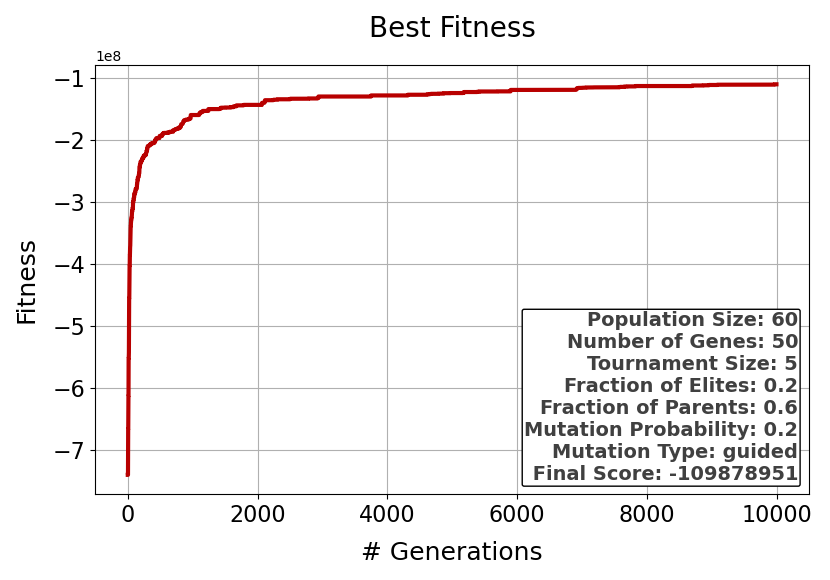
\includegraphics[width=\textwidth]{figures/best_fitness_output_60_50_5_0.2_0.6_0.2_guided.png}
        \caption{From first generation to 10000th generation.}
    \end{subfigure}\hfill
    \begin{subfigure}{0.5\textwidth}
        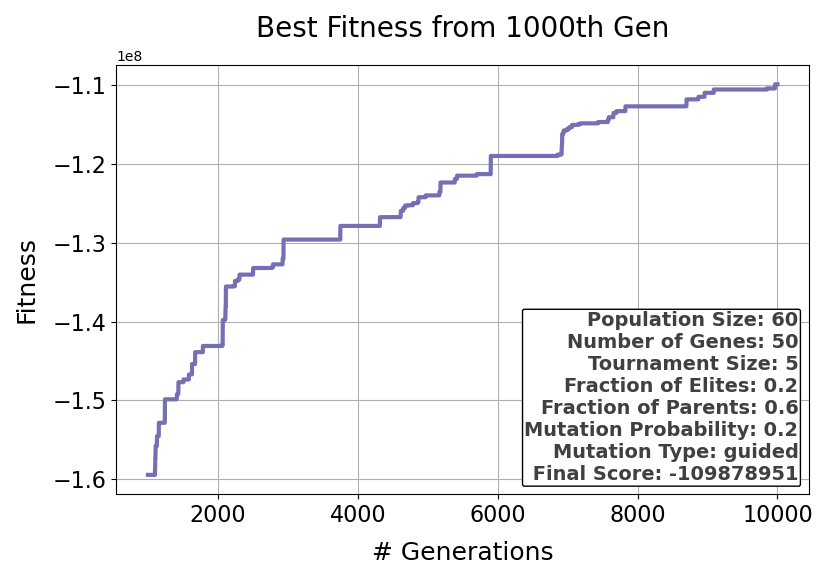
\includegraphics[width=\textwidth]{figures/best_fitness_1000_output_60_50_5_0.2_0.6_0.2_guided.png}
        \caption{From 1000th generation to 10000th generation.}
    \end{subfigure}
    \caption{Fitness curves for 60 individuals.}
\label{fig:60inds}
\end{figure}

The Figure \ref{fig:60inds_image} shows the evolution of the best individual quantitatively for 60 individuals.

\begin{figure}[!htb]
    \centering
    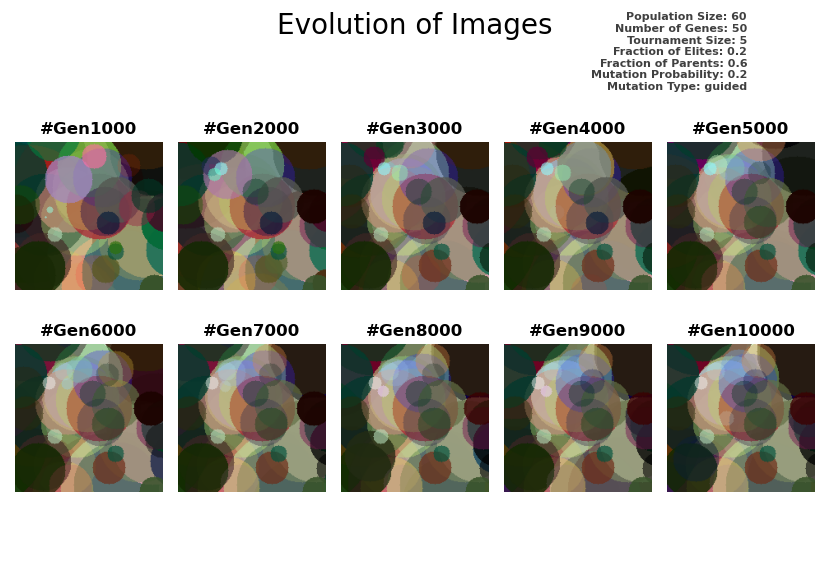
\includegraphics[width=0.9\textwidth]{figures/images_output_60_50_5_0.2_0.6_0.2_guided.png}
    \caption{Quantitative evolution of the best individual in the population for 60 individuals.}
    \label{fig:60inds_image}
\end{figure}

\textbf{Discussion:} The results show that the number of individuals in the population has a significant effect on the performance of the algorithm. It can be deduced that as the number of individuals in the population increases, the algorithm converges to a better solution. This is because the diversity in the population increases as the number of individuals increases.

\subsection{Number of Genes}
Let us first provide necessary plots for the parameter \textless{}num\_genes\textgreater{}.
\subsubsection{15 Genes}
Figure \ref{fig:15genes} shows the plots related to the fitness value of the best individual for 15 genes.

\begin{figure}[H]
    \begin{subfigure}{0.5\textwidth}
        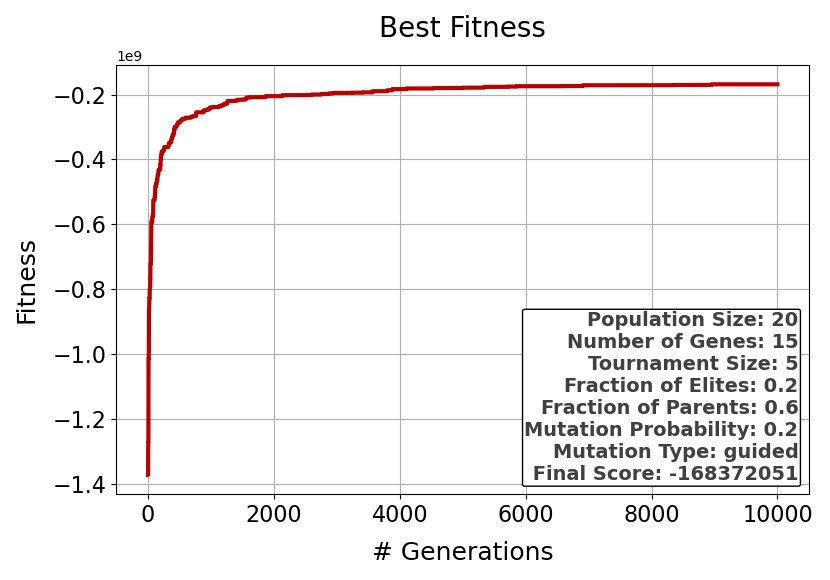
\includegraphics[width=\textwidth]{figures/best_fitness_output_20_15_5_0.2_0.6_0.2_guided.png}
        \caption{From first generation to 10000th generation.}
    \end{subfigure}\hfill
    \begin{subfigure}{0.5\textwidth}
        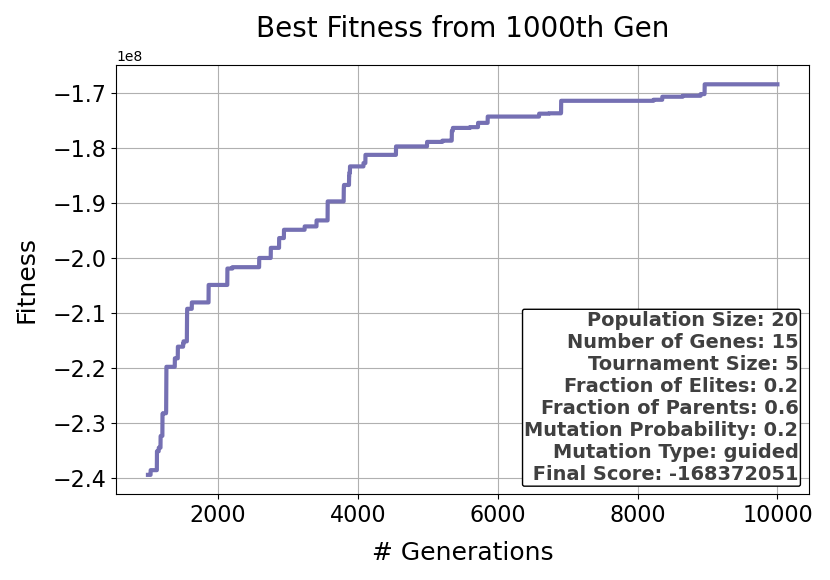
\includegraphics[width=\textwidth]{figures/best_fitness_1000_output_20_15_5_0.2_0.6_0.2_guided.png}
        \caption{From 1000th generation to 10000th generation.}
    \end{subfigure}
    \caption{Fitness curves for 15 genes.}
\label{fig:15genes}
\end{figure}

The Figure \ref{fig:15genes_image} illustrates the evolution of the best individual figuratively for 15 genes.

\begin{figure}[!htb]
    \centering
    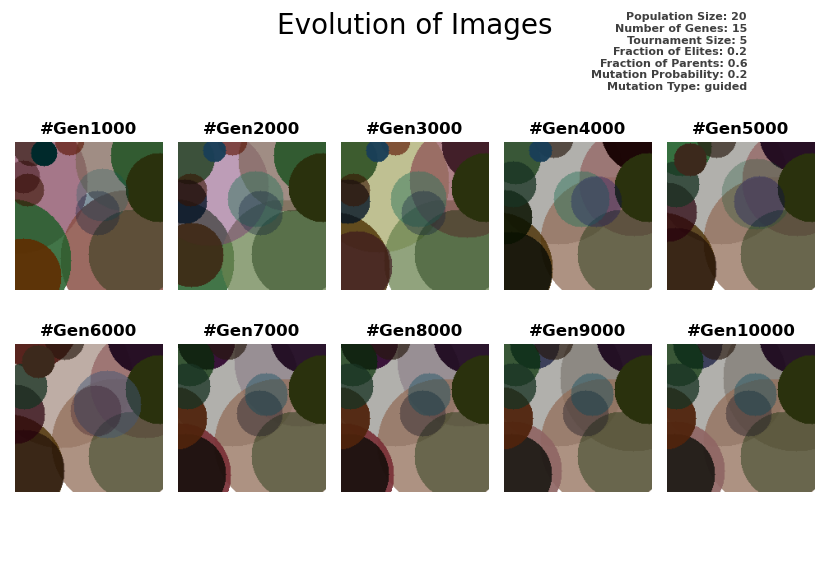
\includegraphics[width=0.9\textwidth]{figures/images_output_20_15_5_0.2_0.6_0.2_guided.png}
    \caption{Quantitative evolution of the best individual in the population for 15 genes.}
    \label{fig:15genes_image}
\end{figure}

\subsubsection{30 Genes}
Figure \ref{fig:30genes} shows the plots related to the fitness value of the best individual for 30 genes.

\begin{figure}[H]
    \begin{subfigure}{0.5\textwidth}
        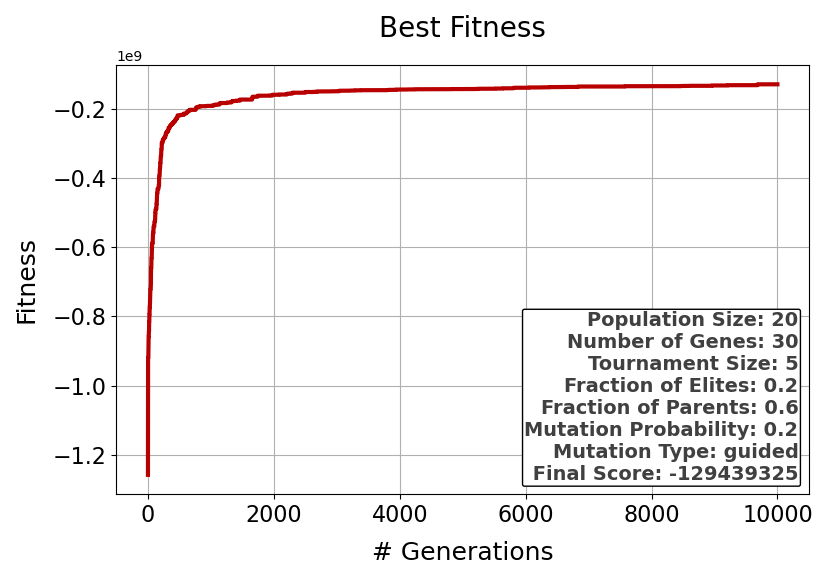
\includegraphics[width=\textwidth]{figures/best_fitness_output_20_30_5_0.2_0.6_0.2_guided.png}
        \caption{From first generation to 10000th generation.}
    \end{subfigure}\hfill
    \begin{subfigure}{0.5\textwidth}
        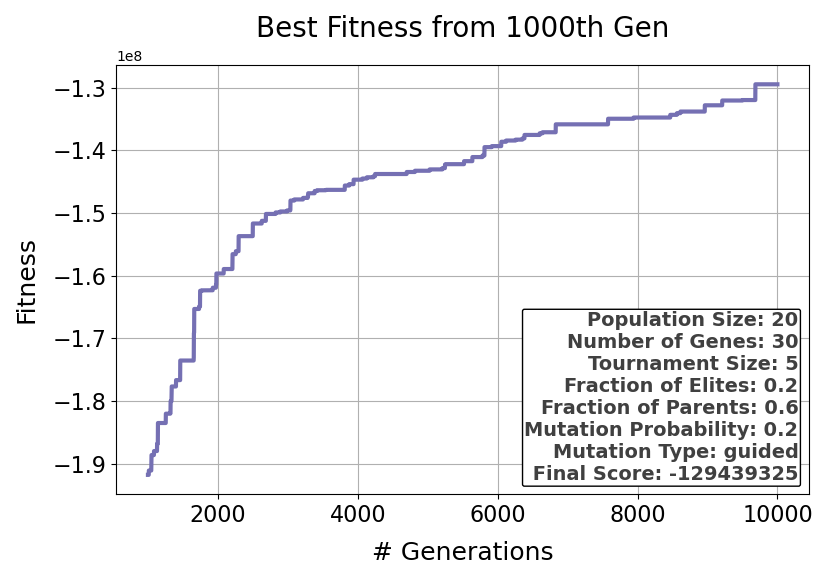
\includegraphics[width=\textwidth]{figures/best_fitness_1000_output_20_30_5_0.2_0.6_0.2_guided.png}
        \caption{From 1000th generation to 10000th generation.}
    \end{subfigure}
    \caption{Fitness curves for 30 genes.}
\label{fig:30genes}
\end{figure}

The Figure \ref{fig:30genes_image} shows the evolution of the best individual figuratively for 30 genes.

\begin{figure}[!htb]
    \centering
    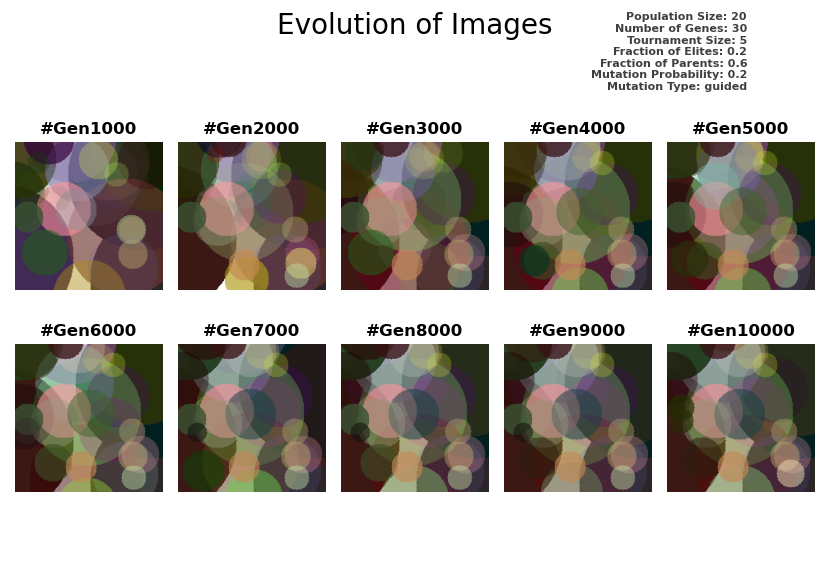
\includegraphics[width=0.9\textwidth]{figures/images_output_20_30_5_0.2_0.6_0.2_guided.png}
    \caption{Quantitative evolution of the best individual in the population for 30 genes.}
    \label{fig:30genes_image}
\end{figure}

\subsubsection{80 Genes}
Figure \ref{fig:80genes} shows the plots related to the fitness value of the best individual for 80 genes.

\begin{figure}[H]
    \begin{subfigure}{0.5\textwidth}
        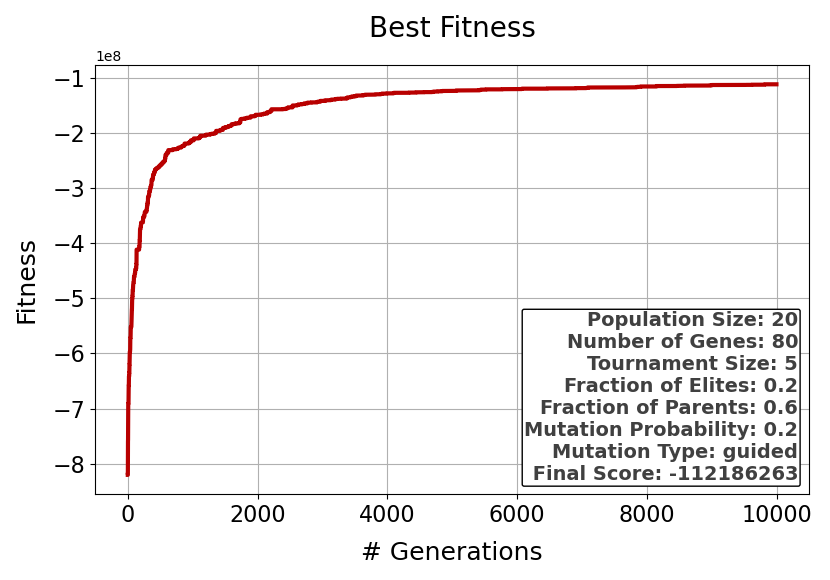
\includegraphics[width=\textwidth]{figures/best_fitness_output_20_80_5_0.2_0.6_0.2_guided.png}
        \caption{From first generation to 10000th generation.}
    \end{subfigure}\hfill
    \begin{subfigure}{0.5\textwidth}
        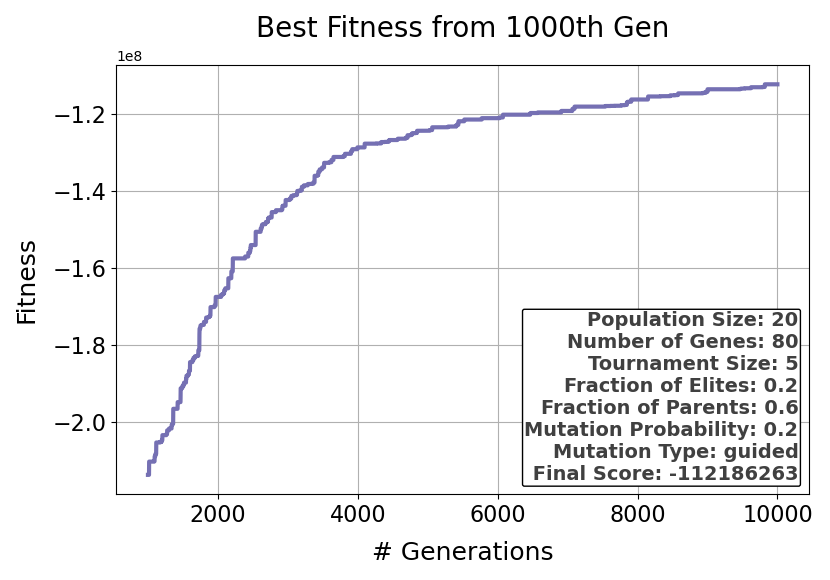
\includegraphics[width=\textwidth]{figures/best_fitness_1000_output_20_80_5_0.2_0.6_0.2_guided.png}
        \caption{From 1000th generation to 10000th generation.}
    \end{subfigure}
    \caption{Fitness curves for 80 genes.}
\label{fig:80genes}
\end{figure}

The Figure \ref{fig:80genes_image} shows the evolution of the best individual figuratively for 80 genes.

\begin{figure}[!htb]
    \centering
    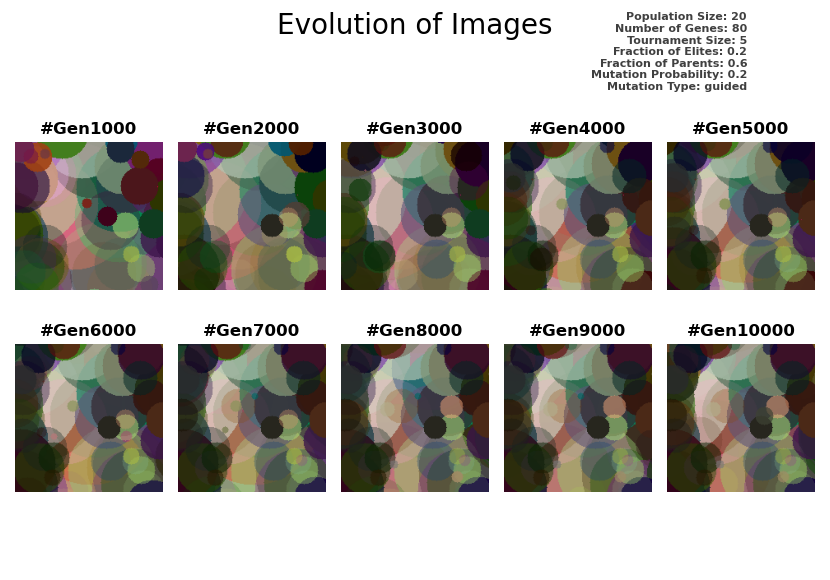
\includegraphics[width=0.9\textwidth]{figures/images_output_20_80_5_0.2_0.6_0.2_guided.png}
    \caption{Quantitative evolution of the best individual in the population for 80 genes.}
    \label{fig:80genes_image}
\end{figure}

\subsubsection{120 Genes}
Figure \ref{fig:120genes} shows the plots related to the fitness value of the best individual for 120 genes.

\begin{figure}[H]
    \begin{subfigure}{0.5\textwidth}
        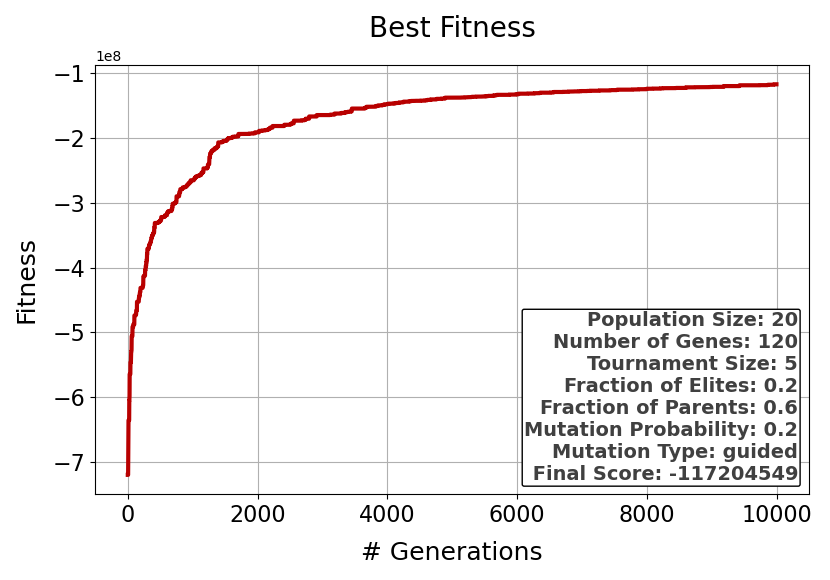
\includegraphics[width=\textwidth]{figures/best_fitness_output_20_120_5_0.2_0.6_0.2_guided.png}
        \caption{From first generation to 10000th generation.}
    \end{subfigure}\hfill
    \begin{subfigure}{0.5\textwidth}
        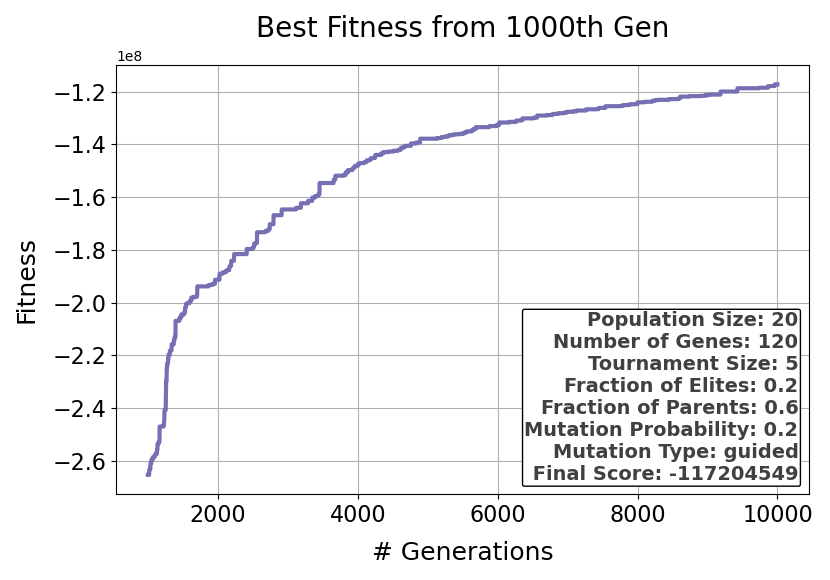
\includegraphics[width=\textwidth]{figures/best_fitness_1000_output_20_120_5_0.2_0.6_0.2_guided.png}
        \caption{From 1000th generation to 10000th generation.}
    \end{subfigure}
    \caption{Fitness curves for 120 genes.}
\label{fig:120genes}
\end{figure}

The Figure \ref{fig:120genes_image} is given for the evolution of the best individual for 120 genes.

\begin{figure}[!htb]
    \centering
    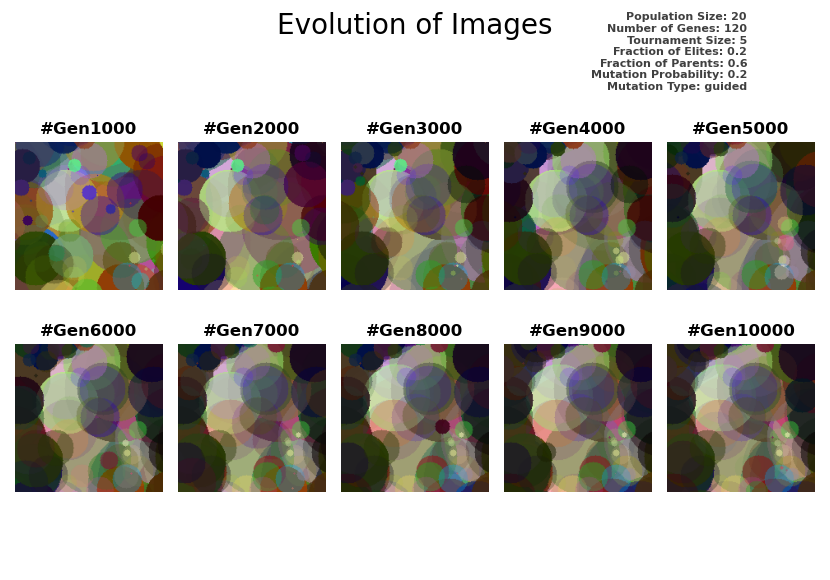
\includegraphics[width=0.9\textwidth]{figures/images_output_20_120_5_0.2_0.6_0.2_guided.png}
    \caption{Quantitative evolution of the best individual in the population for 120 genes.}
    \label{fig:120genes_image}
\end{figure}

\textbf{Discussion:} We see that, as the number of genes in the individual increases, the algorithm converges to a better solution. This is because the number of genes in the individual increases, the search space increases and the algorithm can explore more possibilities. This was somewhat expected since the number of genes in the individual is directly related to "paint brushes" we have in this problem. However, from 80 genes to 120 genes the improvement is not obserable 80 genes converged to a better solution. We can interpret that for 120 genes there need to be more generations to converge to a better solution. So, as the number of genes decreases, the number of generations needed to converge is also decreased. Given we fixed the number of generations, the results are natural in this sense.

\subsection{Tournament Size}
Let us first provide necessary plots for the parameter \textless{}tm\_size\textgreater{}.

\subsubsection{2 Tournament Size}
Figure \ref{fig:2tm} shows the plots related to the fitness value of the best individual for 2 tournament size.

\begin{figure}[H]
    \begin{subfigure}{0.5\textwidth}
        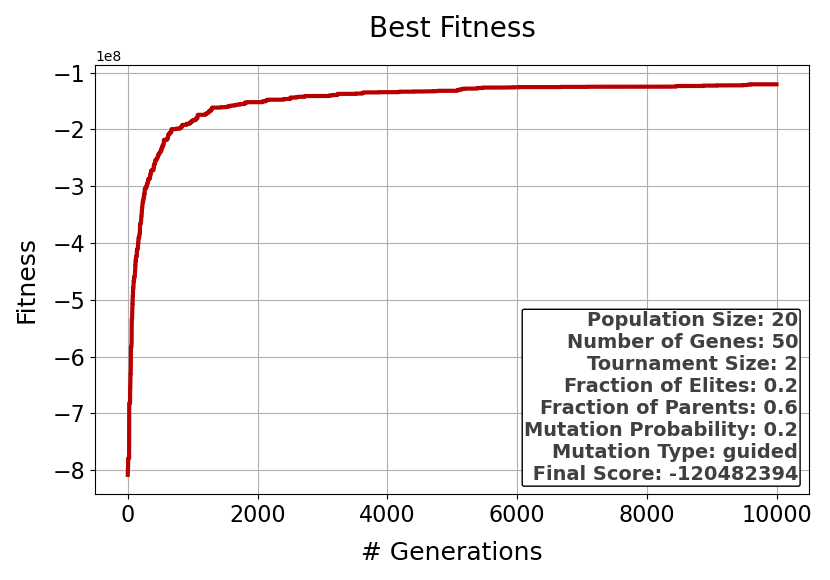
\includegraphics[width=\textwidth]{figures/best_fitness_output_20_50_2_0.2_0.6_0.2_guided.png}
        \caption{From first generation to 10000th generation.}
    \end{subfigure}\hfill
    \begin{subfigure}{0.5\textwidth}
        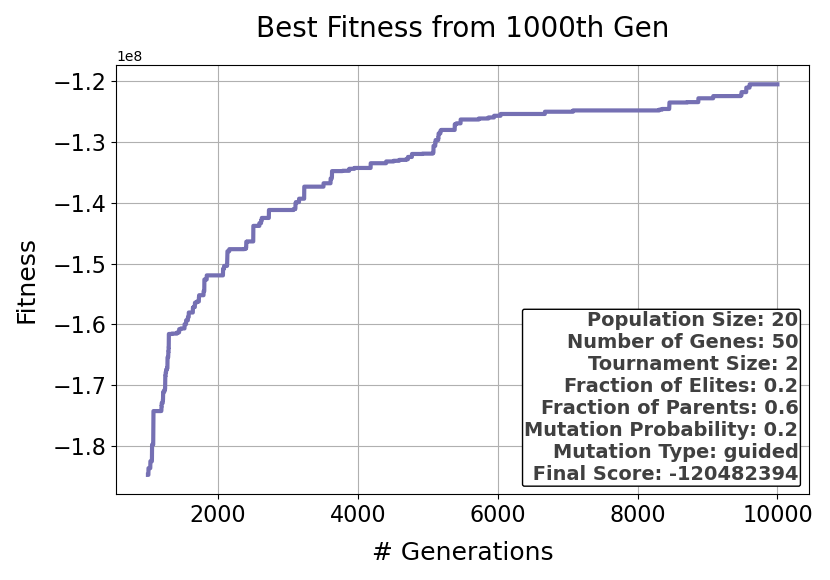
\includegraphics[width=\textwidth]{figures/best_fitness_1000_output_20_50_2_0.2_0.6_0.2_guided.png}
        \caption{From 1000th generation to 10000th generation.}
    \end{subfigure}
    \caption{Fitness curves for 2 tournament size.}
\label{fig:2tm}
\end{figure}

The Figure \ref{fig:2tm_image} shows the evolution of the best individual figuratively for 2 tournament size.

\begin{figure}[!htb]
    \centering
    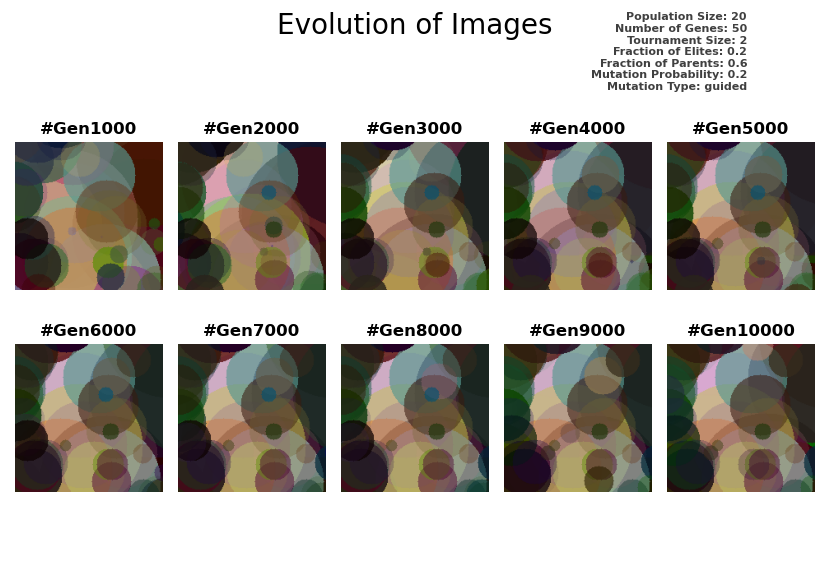
\includegraphics[width=0.9\textwidth]{figures/images_output_20_50_2_0.2_0.6_0.2_guided.png}
    \caption{Quantitative evolution of the best individual in the population for 2 tournament size.}
    \label{fig:2tm_image}
\end{figure}

\subsubsection{8 Tournament Size}
Figure \ref{fig:8tm} shows the plots related to the fitness value of the best individual for 8 tournament size.

\begin{figure}[H]
    \begin{subfigure}{0.5\textwidth}
        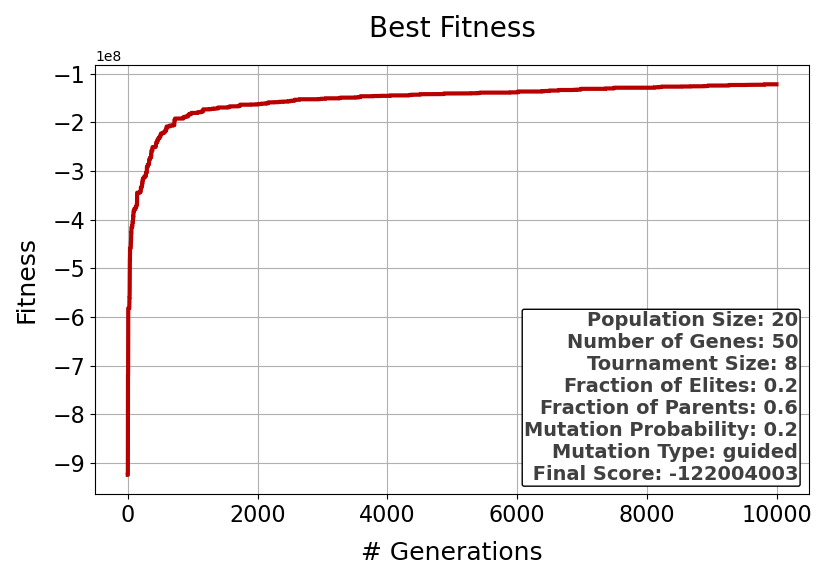
\includegraphics[width=\textwidth]{figures/best_fitness_output_20_50_8_0.2_0.6_0.2_guided.png}
        \caption{From first generation to 10000th generation.}
    \end{subfigure}\hfill
    \begin{subfigure}{0.5\textwidth}
        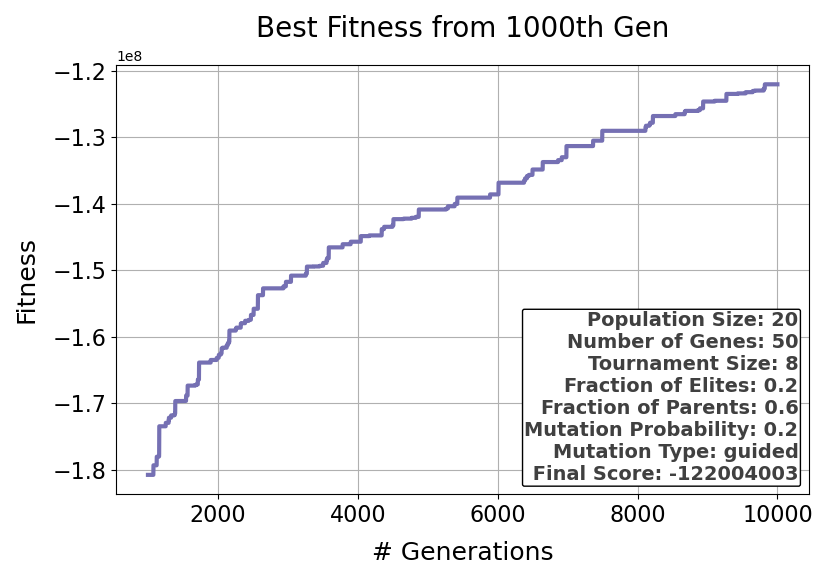
\includegraphics[width=\textwidth]{figures/best_fitness_1000_output_20_50_8_0.2_0.6_0.2_guided.png}
        \caption{From 1000th generation to 10000th generation.}
    \end{subfigure}
    \caption{Fitness curves for 8 tournament size.}
\label{fig:8tm}
\end{figure}

The Figure \ref{fig:8tm_image} shows the evolution of the best individual figuratively for 8 tournament size.

\begin{figure}[!htb]
    \centering
    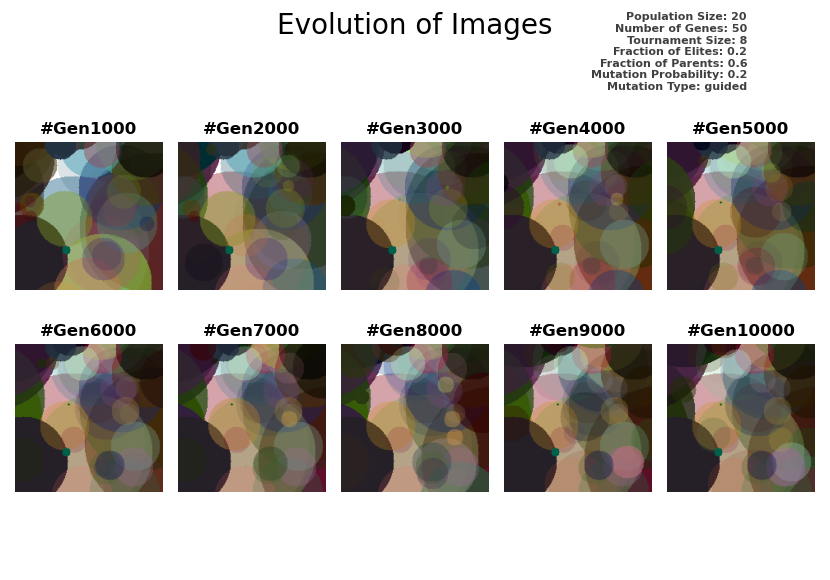
\includegraphics[width=0.9\textwidth]{figures/images_output_20_50_8_0.2_0.6_0.2_guided.png}
    \caption{Quantitative evolution of the best individual in the population for 8 tournament size.}
    \label{fig:8tm_image}
\end{figure}

\subsubsection{16 Tournament Size}
Figure \ref{fig:16tm} shows the plots related to the fitness value of the best individual for 16 tournament size.

\begin{figure}[H]
    \begin{subfigure}{0.5\textwidth}
        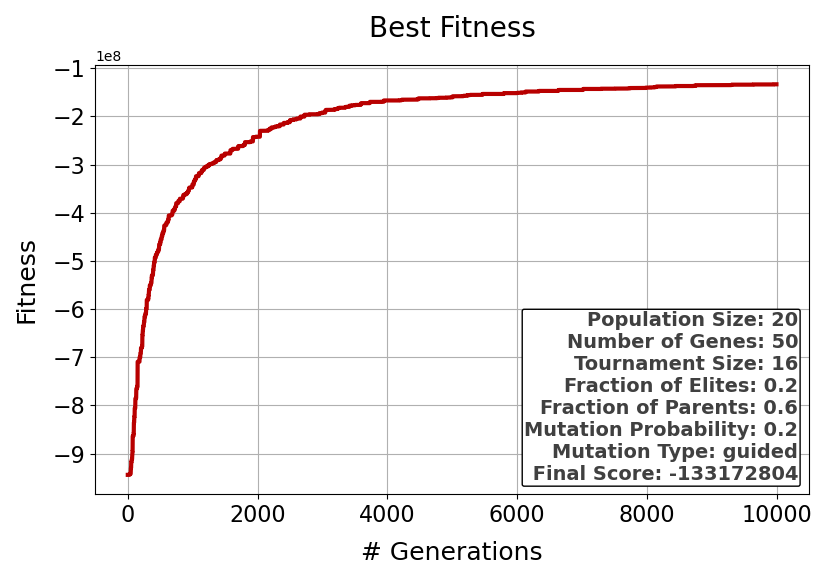
\includegraphics[width=\textwidth]{figures/best_fitness_output_20_50_16_0.2_0.6_0.2_guided.png}
        \caption{From first generation to 10000th generation.}
    \end{subfigure}\hfill
    \begin{subfigure}{0.5\textwidth}
        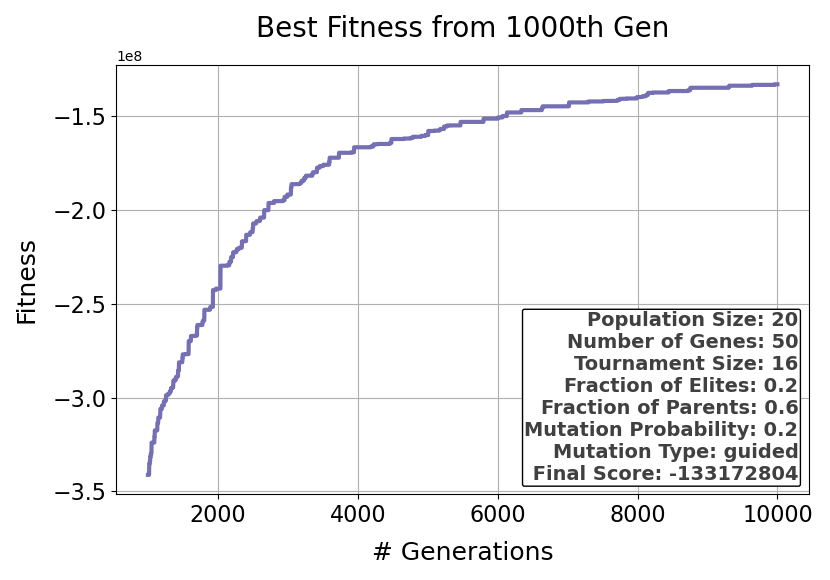
\includegraphics[width=\textwidth]{figures/best_fitness_1000_output_20_50_16_0.2_0.6_0.2_guided.png}
        \caption{From 1000th generation to 10000th generation.}
    \end{subfigure}
    \caption{Fitness curves for 16 tournament size.}
\label{fig:16tm}
\end{figure}

The Figure \ref{fig:16tm_image} shows the evolution of the best individual figuratively for 16 tournament size.

\begin{figure}[!htb]
    \centering
    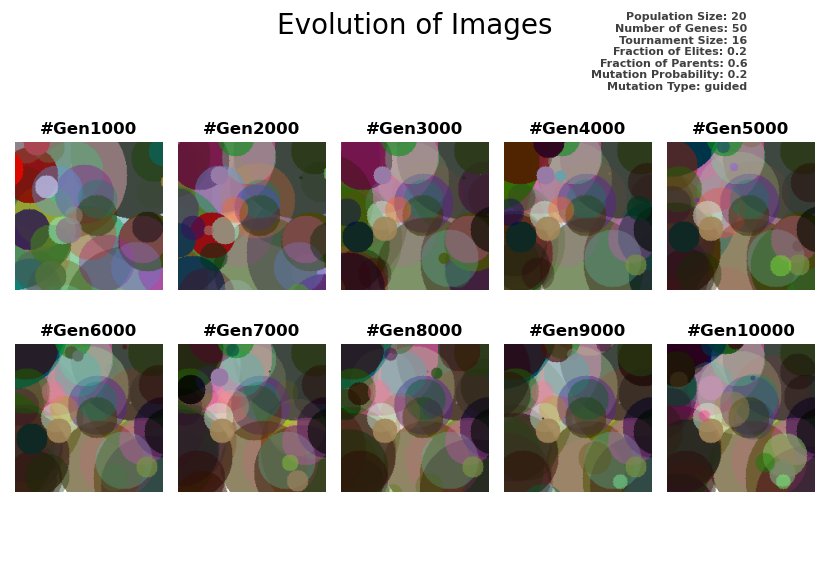
\includegraphics[width=0.9\textwidth]{figures/images_output_20_50_16_0.2_0.6_0.2_guided.png}
    \caption{Quantitative evolution of the best individual in the population for 16 tournament size.}
    \label{fig:16tm_image}
\end{figure}

\textbf{Discussion:} From the results we see that the best tournament size selection for this parameter space was 5. This means there are no linear relationship between the tournament size and the performance of the algorithm. As the tournament size increases too much the diversity decreased. It can be said that tournament size is a hyperparameter that needs to be tuned for the specific problem. If we change the other parameters such as number of individuals, number of genes, etc. the best tournament size would change.

\subsection{Number of Individuals Advancing to Next Generation}
Let us first provide necessary plots for the parameter \textless{}frac\_elites\textgreater{}.

\subsubsection{0.04 Fraction of Elites}
Figure \ref{fig:0.04elites} shows the plots related to the fitness value of the best individual for 0.04 fraction of elites.

\begin{figure}[H]
    \begin{subfigure}{0.5\textwidth}
        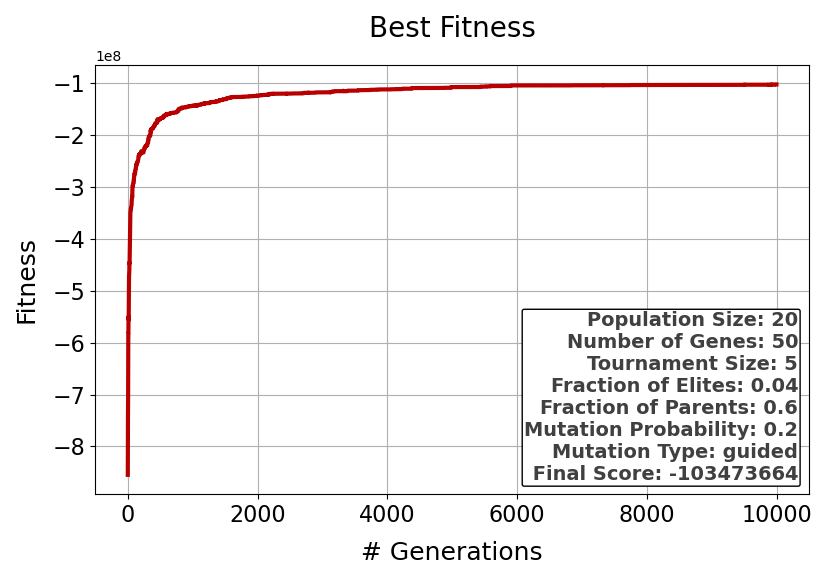
\includegraphics[width=\textwidth]{figures/best_fitness_output_20_50_5_0.04_0.6_0.2_guided.png}
        \caption{From first generation to 10000th generation.}
    \end{subfigure}\hfill
    \begin{subfigure}{0.5\textwidth}
        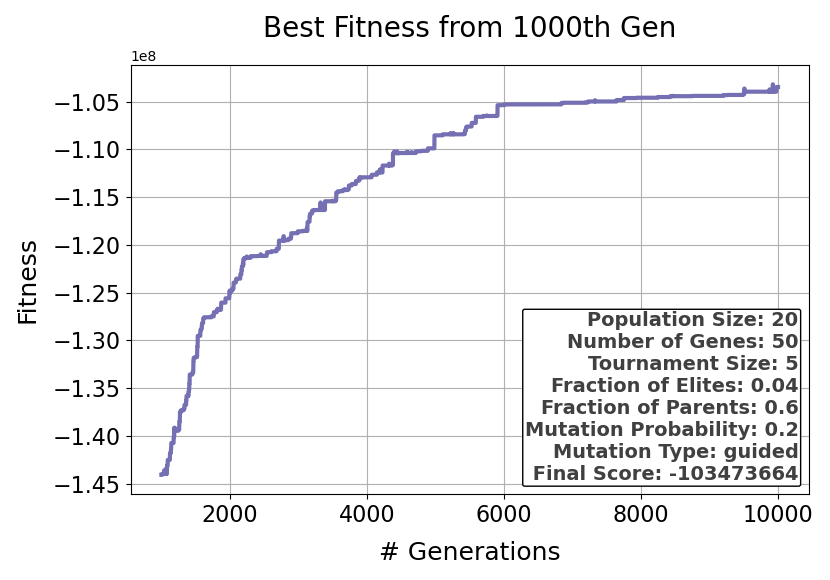
\includegraphics[width=\textwidth]{figures/best_fitness_1000_output_20_50_5_0.04_0.6_0.2_guided.png}
        \caption{From 1000th generation to 10000th generation.}
    \end{subfigure}
    \caption{Fitness curves for 0.04 fraction of elites.}
\label{fig:0.04elites}
\end{figure}

The Figure \ref{fig:0.04elites_image} shows the evolution of the best individual figuratively for 0.04 fraction of elites.

\begin{figure}[!htb]
    \centering
    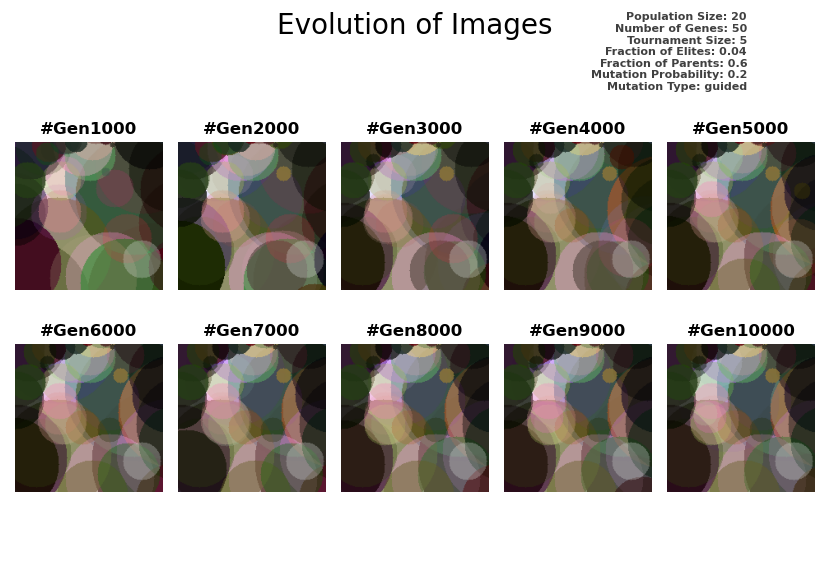
\includegraphics[width=0.9\textwidth]{figures/images_output_20_50_5_0.04_0.6_0.2_guided.png}
    \caption{Quantitative evolution of the best individual in the population for 0.04 fraction of elites.}
    \label{fig:0.04elites_image}
\end{figure}

\subsubsection{0.35 Fraction of Elites}

Figure \ref{fig:0.35elites} shows the plots related to the fitness value of the best individual for 0.35 fraction of elites.

\begin{figure}[H]
    \begin{subfigure}{0.5\textwidth}
        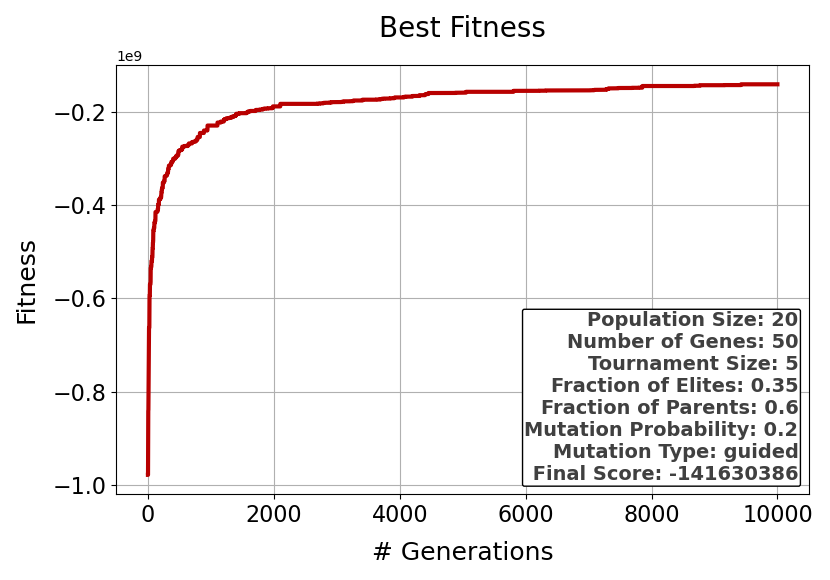
\includegraphics[width=\textwidth]{figures/best_fitness_output_20_50_5_0.35_0.6_0.2_guided.png}
        \caption{From first generation to 10000th generation.}
    \end{subfigure}\hfill
    \begin{subfigure}{0.5\textwidth}
        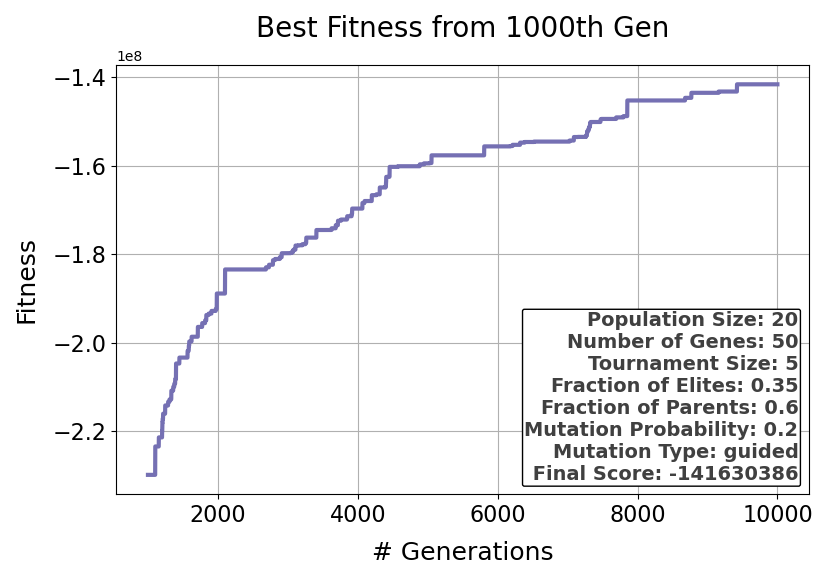
\includegraphics[width=\textwidth]{figures/best_fitness_1000_output_20_50_5_0.35_0.6_0.2_guided.png}
        \caption{From 1000th generation to 10000th generation.}
    \end{subfigure}
    \caption{Fitness curves for 0.35 fraction of elites.}
\label{fig:0.35elites}
\end{figure}

The Figure \ref{fig:0.35elites_image} shows the evolution of the best individual figuratively for 0.35 fraction of elites.

\begin{figure}[!htb]
    \centering
    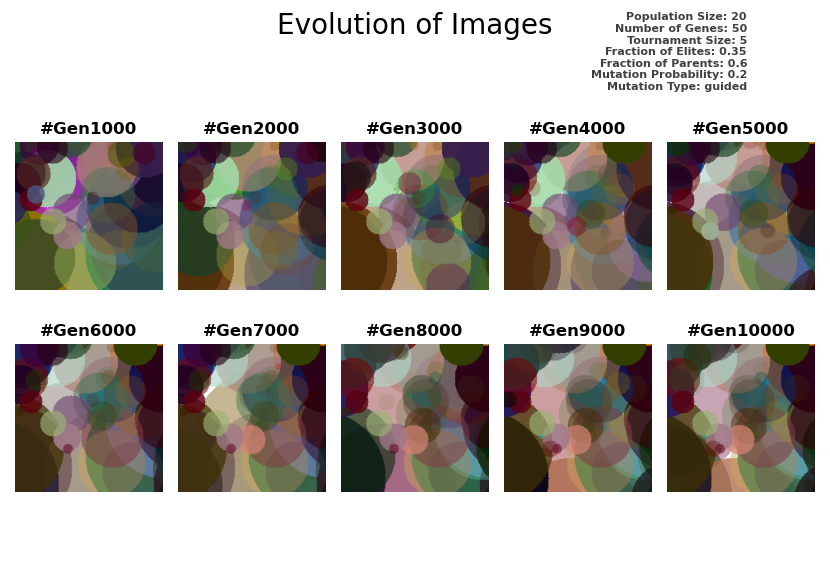
\includegraphics[width=0.9\textwidth]{figures/images_output_20_50_5_0.35_0.6_0.2_guided.png}
    \caption{Quantitative evolution of the best individual in the population for 0.35 fraction of elites.}
    \label{fig:0.35elites_image}
\end{figure}

\textbf{Discussion:} The results indicates that the best selection for the fraction of elites is 0.04. We may interpret this as the algorithm needs more diversity in the population to converge to a better solution. On the other hand this implied follows, as the number of elites decreases the parents selected are shifts to a better group of individuals. So, it is hard to tell the number of elites is decoupled from the other parameters. If we select parents first from the best individuals and then from the rest of the population, the best fraction of elites would change.

\subsection{Number of Parents Used In Crossover}

Let us first provide necessary plots for the parameter \textless{}frac\_parents\textgreater{}.

\subsubsection{0.15 Fraction of Parents}
The plots about to the fitness metric of the best individual for 0.15 fraction of parents in Figure \ref{fig:0.15parents}.

\begin{figure}[H]
    \begin{subfigure}{0.5\textwidth}
        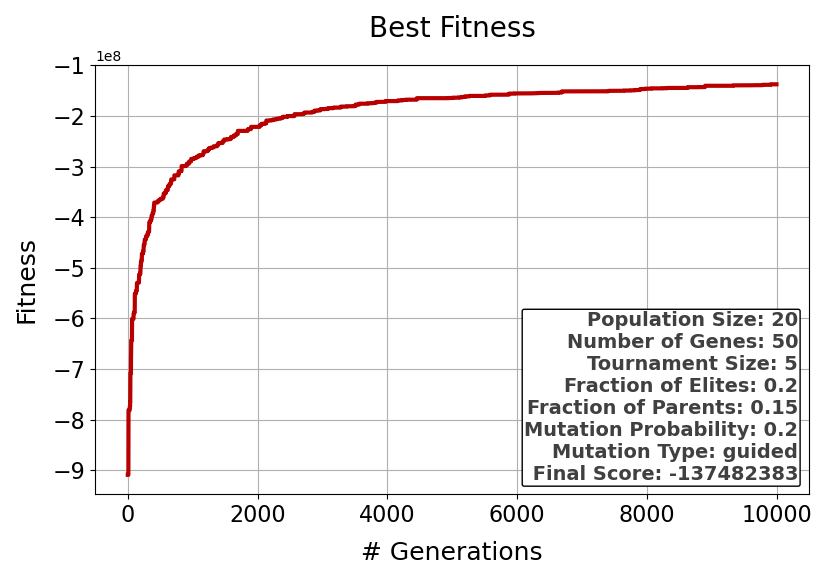
\includegraphics[width=\textwidth]{figures/best_fitness_output_20_50_5_0.2_0.15_0.2_guided.png}
        \caption{From first generation to 10000th generation.}
    \end{subfigure}\hfill
    \begin{subfigure}{0.5\textwidth}
        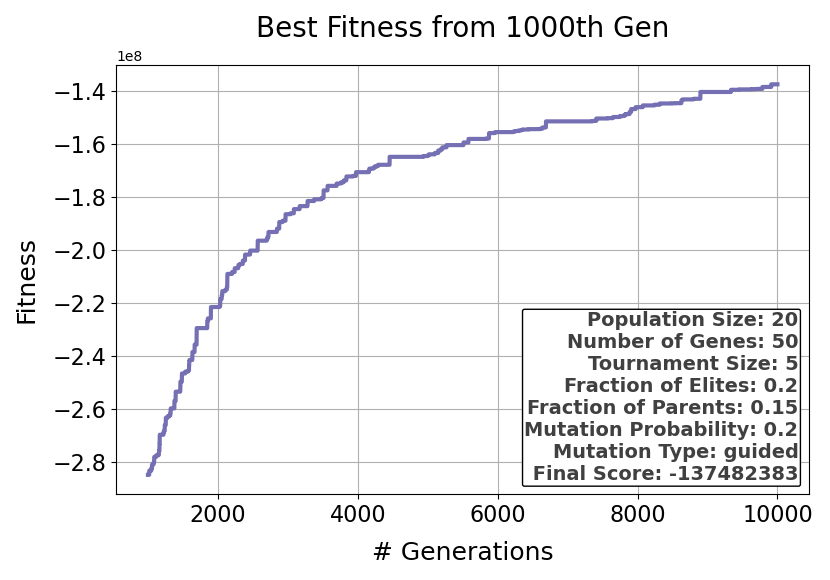
\includegraphics[width=\textwidth]{figures/best_fitness_1000_output_20_50_5_0.2_0.15_0.2_guided.png}
        \caption{From 1000th generation to 10000th generation.}
    \end{subfigure}
    \caption{Fitness curves for 0.15 fraction of parents.}
\label{fig:0.15parents}
\end{figure}

The evolution of the best individual for 0.15 fraction of parents is given in Figure \ref{fig:0.15parents_image}.

\begin{figure}[!htb]
    \centering
    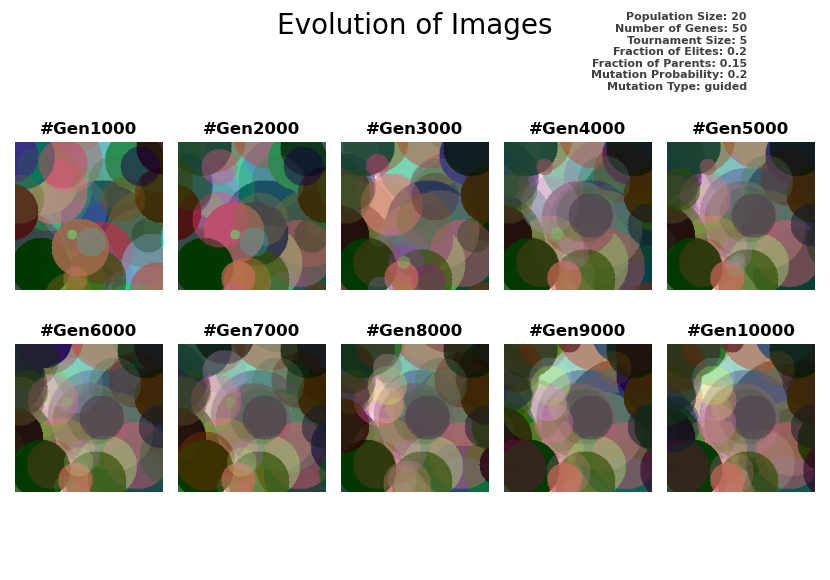
\includegraphics[width=0.9\textwidth]{figures/images_output_20_50_5_0.2_0.15_0.2_guided.png}
    \caption{Quantitative evolution of the best individual in the population for 0.15 fraction of parents.}
    \label{fig:0.15parents_image}
\end{figure}

\subsubsection{0.3 Fraction of Parents}

The plots about to the fitness metric of the best individual for 0.3 fraction of parents in Figure \ref{fig:0.3parents}.
\begin{figure}[H]
    \begin{subfigure}{0.5\textwidth}
        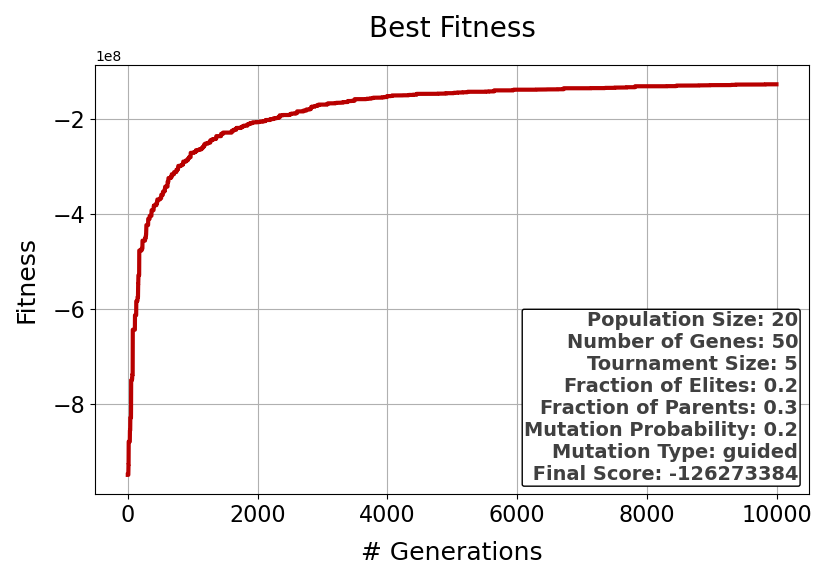
\includegraphics[width=\textwidth]{figures/best_fitness_output_20_50_5_0.2_0.3_0.2_guided.png}
        \caption{From first generation to 10000th generation.}
    \end{subfigure}\hfill
    \begin{subfigure}{0.5\textwidth}
        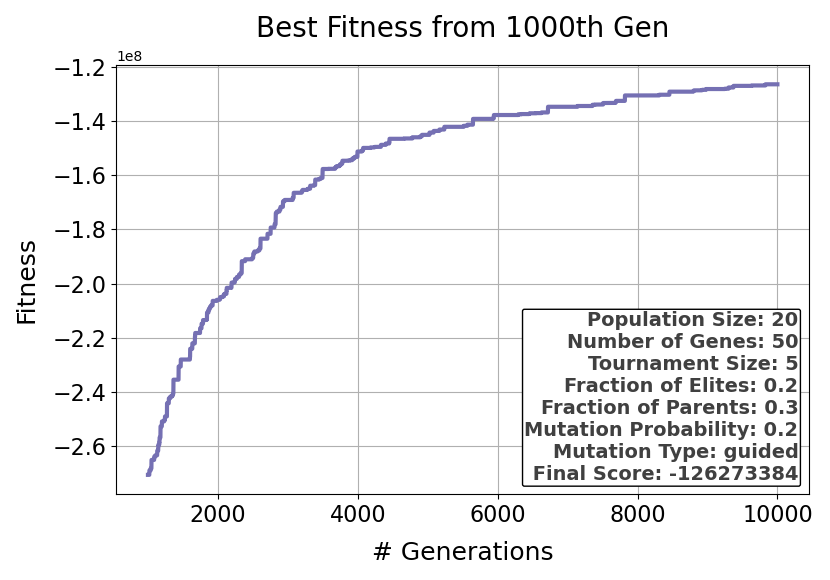
\includegraphics[width=\textwidth]{figures/best_fitness_1000_output_20_50_5_0.2_0.3_0.2_guided.png}
        \caption{From 1000th generation to 10000th generation.}
    \end{subfigure}
    \caption{Fitness curves for 0.3 fraction of parents.}
\label{fig:0.3parents}
\end{figure}

The evolution of the best individual for 0.3 fraction of parents is given in Figure \ref{fig:0.3parents_image}.
\begin{figure}[!htb]
    \centering
    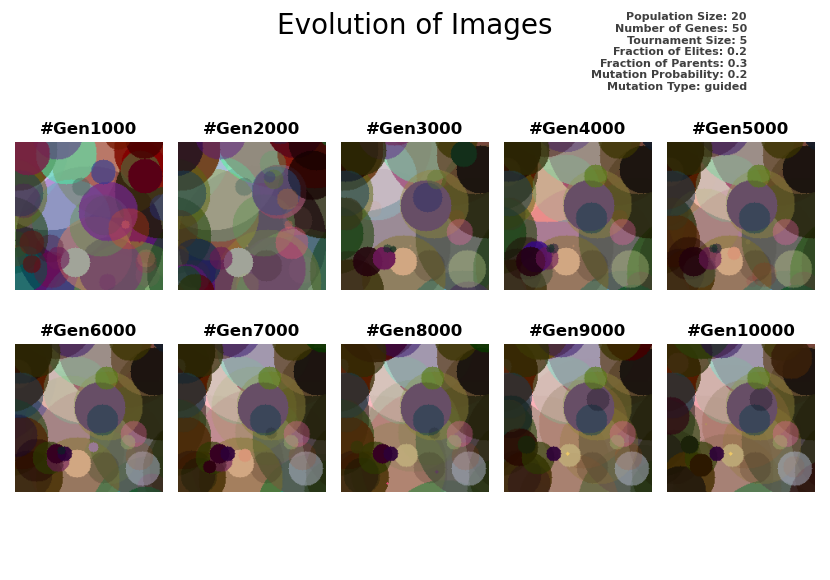
\includegraphics[width=0.9\textwidth]{figures/images_output_20_50_5_0.2_0.3_0.2_guided.png}
    \caption{Quantitative evolution of the best individual in the population for 0.3 fraction of parents.}
    \label{fig:0.3parents_image}
\end{figure}

\subsubsection{0.75 Fraction of Parents}

The plots about to the fitness metric of the best individual for 0.75 fraction of parents in Figure \ref{fig:0.75parents}.
\begin{figure}[H]
    \begin{subfigure}{0.5\textwidth}
        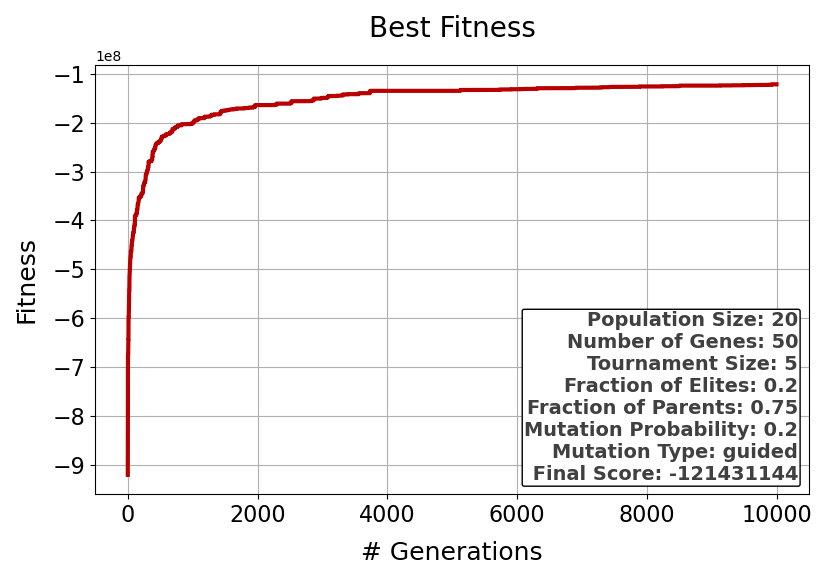
\includegraphics[width=\textwidth]{figures/best_fitness_output_20_50_5_0.2_0.75_0.2_guided.png}
        \caption{From first generation to 10000th generation.}
    \end{subfigure}\hfill
    \begin{subfigure}{0.5\textwidth}
        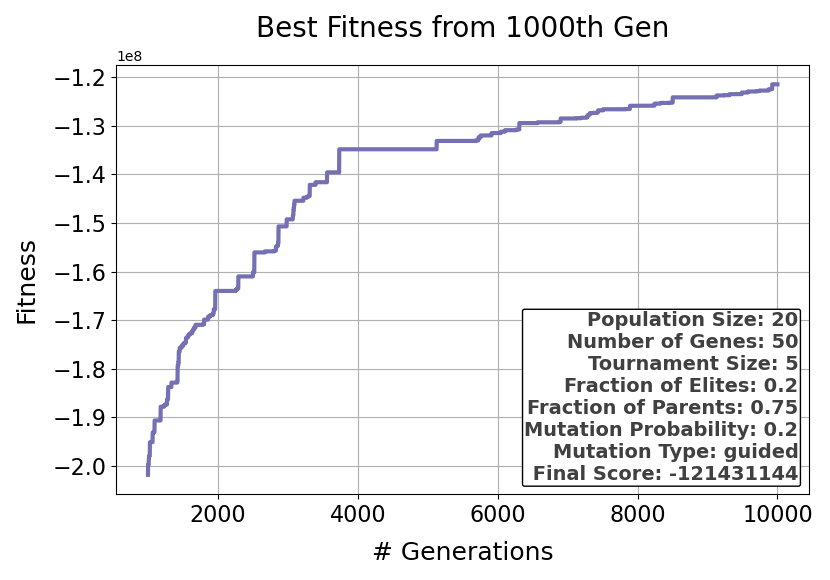
\includegraphics[width=\textwidth]{figures/best_fitness_1000_output_20_50_5_0.2_0.75_0.2_guided.png}
        \caption{From 1000th generation to 10000th generation.}
    \end{subfigure}
    \caption{Fitness curves for 0.75 fraction of parents.}
\label{fig:0.75parents}
\end{figure}

The evolution of the best individual for 0.75 fraction of parents is given in Figure \ref{fig:0.75parents_image}.

\begin{figure}[!htb]
    \centering
    \includegraphics[width=0.9\textwidth]{figures/images_output_20_50_5_0.2_0.75_0.2_guided.png}
    \caption{Quantitative evolution of the best individual in the population for 0.75 fraction of parents.}
    \label{fig:0.75parents_image}
\end{figure}

\textbf{Discussion:} The results show that the best selection for the fraction of parents is 0.6. This means that the algorithm needs to select parents from a wide range of individuals to converge to a better solution. This is because the diversity in the population is important for the algorithm to explore more possibilities. If the algorithm selects parents from a small group of individuals, the algorithm may converge to a local minimum. On the other hand for the case of 0.75 fraction of parents, we see that increasing the fraction of parents did not help. We may interpret this result as the algorithm needs to select parents from a wide range of individuals but not from the whole population.


\subsection{Mutation Probability}
Let us first provide necessary plots for the parameter \textless{}mutation\_prob\textgreater{}.

\subsubsection{0.1 Mutation Probability}
The plots about to the fitness metric of the best individual for 0.1 mutation probability in Figure \ref{fig:0.1mutation}.

\begin{figure}[H]
    \begin{subfigure}{0.5\textwidth}
        \includegraphics[width=\textwidth]{figures/best_fitness_output_20_50_5_0.2_0.6_0.1_guided.png}
        \caption{From first generation to 10000th generation.}
    \end{subfigure}\hfill
    \begin{subfigure}{0.5\textwidth}
        \includegraphics[width=\textwidth]{figures/best_fitness_1000_output_20_50_5_0.2_0.6_0.1_guided.png}
        \caption{From 1000th generation to 10000th generation.}
    \end{subfigure}
    \caption{Fitness curves for 0.1 mutation probability.}
\label{fig:0.1mutation}
\end{figure}

The evolution of the best individual for 0.1 mutation probability is given in Figure \ref{fig:0.1mutation_image}.
\begin{figure}[!htb]
    \centering
    \includegraphics[width=0.9\textwidth]{figures/images_output_20_50_5_0.2_0.6_0.1_guided.png}
    \caption{Quantitative evolution of the best individual in the population for 0.1 mutation probability.}
    \label{fig:0.1mutation_image}
\end{figure}

\subsubsection{0.4 Mutation Probability}
The plots about to the fitness metric of the best individual for 0.4 mutation probability in Figure \ref{fig:0.4mutation}.

\begin{figure}[H]
    \begin{subfigure}{0.5\textwidth}
        \includegraphics[width=\textwidth]{figures/best_fitness_output_20_50_5_0.2_0.6_0.4_guided.png}
        \caption{From first generation to 10000th generation.}
    \end{subfigure}\hfill
    \begin{subfigure}{0.5\textwidth}
        \includegraphics[width=\textwidth]{figures/best_fitness_1000_output_20_50_5_0.2_0.6_0.4_guided.png}
        \caption{From 1000th generation to 10000th generation.}
    \end{subfigure}
    \caption{Fitness curves for 0.4 mutation probability.}
\label{fig:0.4mutation}
\end{figure}

The evolution of the best individual for 0.4 mutation probability is given in Figure \ref{fig:0.4mutation_image}.

\begin{figure}[!htb]
    \centering
    \includegraphics[width=0.9\textwidth]{figures/images_output_20_50_5_0.2_0.6_0.4_guided.png}
    \caption{Quantitative evolution of the best individual in the population for 0.4 mutation probability.}
    \label{fig:0.4mutation_image}
\end{figure}

\subsubsection{0.75 Mutation Probability}

The plots about to the fitness metric of the best individual for 0.75 mutation probability in Figure \ref{fig:0.75mutation}.

\begin{figure}[H]
    \begin{subfigure}{0.5\textwidth}
        \includegraphics[width=\textwidth]{figures/best_fitness_output_20_50_5_0.2_0.6_0.75_guided.png}
        \caption{From first generation to 10000th generation.}
    \end{subfigure}\hfill
    \begin{subfigure}{0.5\textwidth}
        \includegraphics[width=\textwidth]{figures/best_fitness_1000_output_20_50_5_0.2_0.6_0.75_guided.png}
        \caption{From 1000th generation to 10000th generation.}
    \end{subfigure}
    \caption{Fitness curves for 0.75 mutation probability.}
\label{fig:0.75mutation}
\end{figure}

The evolution of the best individual for 0.75 mutation probability is given in Figure \ref{fig:0.75mutation_image}.
\begin{figure}[!htb]
    \centering
    \includegraphics[width=0.9\textwidth]{figures/images_output_20_50_5_0.2_0.6_0.75_guided.png}
    \caption{Quantitative evolution of the best individual in the population for 0.75 mutation probability.}
    \label{fig:0.75mutation_image}
\end{figure}

\textbf{Discussion:} The results show that the best selection for the mutation probability is 0.2. This tells us two things. First, if the mutation probability is too low, the algorithm may not be able to explore the search space effectively. Second, if the mutation probability is too high, the algorithm may not be able to converge to a better solution. This is because if the mutation probability is too high, the algorithm may not be able to preserve the good genes in the population. So, the mutation probability is a hyperparameter that needs to be tuned for the specific problem.

\subsection{Mutation Type}

Let us first provide necessary plots for the parameter \textless{}mutation\_type\textgreater{}.

\subsubsection{Unguided Mutation}
The plots about to the fitness metric of the best individual for unguided mutation in Figure \ref{fig:unguided}.

\begin{figure}[H]
    \begin{subfigure}{0.5\textwidth}
        \includegraphics[width=\textwidth]{figures/best_fitness_output_20_50_5_0.2_0.6_0.2_unguided.png}
        \caption{From first generation to 10000th generation.}
    \end{subfigure}\hfill
    \begin{subfigure}{0.5\textwidth}
        \includegraphics[width=\textwidth]{figures/best_fitness_1000_output_20_50_5_0.2_0.6_0.2_unguided.png}
        \caption{From 1000th generation to 10000th generation.}
    \end{subfigure}
    \caption{Fitness curves for unguided mutation.}
\label{fig:unguided}
\end{figure}

The evolution of the best individual for unguided mutation is given in Figure \ref{fig:unguided_image}.

\begin{figure}[!htb]
    \centering
    \includegraphics[width=0.9\textwidth]{figures/images_output_20_50_5_0.2_0.6_0.2_unguided.png}
    \caption{Quantitative evolution of the best individual in the population for unguided mutation.}
    \label{fig:unguided_image}
\end{figure}

\textbf{Discussion:} It is quite obvious that if the mutation is unguided, the algorithm cannot converge to a better solution. This is because the mutation become reinitialization of the gene. So, the mutation loses its evolutionary meaning.

\section{Discussion - Suggestions}

There are three suggestions, based on our observations and results, that can be made to improve the performance of the algorithm.

\subsection{Search Space Narrowing}

\subsection{Dynamic Mutation Probability}

\subsection{Dynamic Mutation Type}

\section*{Appendix}
The code set used throughout this homework is provided as follows. 

% \lstinputlisting[language=Python]{../parameter_sweep_hw2.py}

% \lstinputlisting[language=Python]{../analysis.py}


%--------------------------------------BIBLIOGRAFIA-------------------------------------------
\nocite{*} 


\end{document}

\begin{figure}[!htb]
    \centering
    \includegraphics[width=0.6\textwidth]{figures/partial_der.jpg}
    \caption{Partial derivative calculation steps for Tanh, Sigmoid and ReLU activation functions.}
    \label{partial_der}
\end{figure}

\begin{figure}[!htb]
    \begin{subfigure}{0.5\textwidth}
        \includegraphics[width=\textwidth]{figures/q2_kernels.png}
        \caption{Kernels}
    \end{subfigure}\hfill
    \begin{subfigure}{0.5\textwidth}
        \includegraphics[width=\textwidth]{figures/q2_zero_input.png}
        \caption{Input set for number zero.}
    \end{subfigure}
    \caption{Kernel and input for number zero.}
    \label{fig:kernel_input}
\end{figure}